\section{Moments}

\subsection{Expectation}

  \begin{definition}[Expectation]
    \label{def:expectation}
    Given a \hyperref[def:probability-space]{probability space} $(\Omega, \mathcal{F}, \mathbb{P})$ and a \hyperref[def:random-variable]{random variable} $X: \Omega \to \mathbb{R}$, the \textbf{expectation} of $X$ is 
    \begin{equation}
      \mathbb{E}[X] \coloneqq \int_\Omega X \, d\mathbb{P}
    \end{equation}
		when the integral is defined.\footnote{Writing $X = X^+ - X^-$, where $X^+ = \max(X, 0)$ and $X^- = - \min(X, 0)$, this is $\mathbb{E}[X] = \mathbb{E}[X^+] - \mathbb{E}[X^-]$ which is well-defined as long as we don't have ``$\infty - \infty$.'' } 
		\begin{enumerate}
		  \item \textit{Discrete Random Variables}. For discrete random variables, 
				\begin{equation}
					\mathbb{E}[X] = \sum_{x \in \mathcal{X}} x \, \mathbb{P}(X = x)
				\end{equation}

			\item \textit{Continuous Random Variables}. If $X$ takes values in $\mathbb{R}$, then 
				\begin{equation}
					\mathbb{E}[X] = \int_{-\infty}^\infty x f_X (x)\,dx 
				\end{equation}
		\end{enumerate}
  \end{definition}
  \begin{proof}
    It suffices to prove the formulas for $X \geq 0$; the general case follows by applying them to $X^+$ and $X^-$ and subtracting (which is well-defined exactly when we don't have $\infty - \infty$). 

    \textit{Discrete.} For $x \in \mathcal{X}$ let $E_x = X^{-1} (\{x\}) \subset \Omega$. These are countably many disjoint sets that cover $\Omega$, and $X = x$ on $E_x$, so 
    \begin{equation}
      \int_{E_x} X \, d\mathbb{P} = x \cdot \mathbb{P}(E_x) = x \cdot \mathbb{P}(X = x)
    \end{equation}
    By \hyperref[mt-thm:countable-additivity-of-integration]{countable additivity of the integral} over the partition $\{E_x\}_{x \in \mathcal{X}}$, 
    \begin{equation}
      \mathbb{E}[X] = \int_\Omega X \, d\mathbb{P} = \sum_{x \in \mathcal{X}} \int_{E_x} X \, d\mathbb{P} = \sum_{x \in \mathcal{X}} x \, \mathbb{P}(X = x)
    \end{equation}

    \textit{Continuous.} By \hyperref[thm:lotus]{LOTUS} with $g = \mathrm{id}$, $\mathbb{E}[X] = \int_\Omega X \,d\mathbb{P} = \int_{\mathbb{R}} x \,d\mathbb{P}_X (x)$. Since $X$ is continuous, $\mathbb{P}_X (B) = \int_B f_X \,d\lambda$ for every Borel $B$, i.e. $\int 1_B \,d\mathbb{P}_X = \int 1_B f_X \,d\lambda$. By linearity this holds for non-negative simple functions in place of $1_B$, and by the monotone convergence theorem (approximating $x \mapsto x$ on $[0, \infty)$ from below by simple functions) it holds for $x \mapsto x$. Therefore, 
    \begin{equation}
      \mathbb{E}[X] = \int_{\mathbb{R}} x \,d\mathbb{P}_X (x) = \int_{\mathbb{R}} x f_X (x) \,d\lambda (x) = \int_{-\infty}^\infty x f_X (x) \,dx
    \end{equation}
  \end{proof}

  Note that the reason why expectations of the form $\infty - \infty$ are indeterminate is because of the \hyperref[real-thm:riemann-rearrangement-theorem]{Riemann rearrangement theorem}, which says that a conditionally convergent series can be rearranged to converge to any real number. 

  \begin{theorem}[Tail Sum Formula]
    \label{thm:tail-sum-formula}
		Let $X$ be a non-negative random variable taking values in $\mathbb{R}$. Then, 
		\begin{equation}
			\mathbb{E}[X] = \int_0^\infty \mathbb{P}(X > x) \,dx = \int_0^\infty (1 - F_X (x)) \,dx
		\end{equation}
		Particularly, 
		\begin{enumerate}
		  \item \textit{Discrete Random Variables}. 
				\begin{equation}
					\mathbb{E}[X] = \sum_{k=1}^\infty \mathbb{P}(X \geq k)
				\end{equation}

			\item \textit{Continuous Random Variables}. 
				\begin{equation}
					\mathbb{E}[X] = \int_0^\infty \mathbb{P}(X \geq x) \,dx 
				\end{equation}
		\end{enumerate}
  \end{theorem}
  \begin{proof}
    For every $\omega \in \Omega$, since $X(\omega) \geq 0$, 
    \begin{equation}
      X(\omega) = \int_0^\infty 1_{\{x < X(\omega)\}} \,dx
    \end{equation}
    The function $(\omega, x) \mapsto 1_{\{x < X(\omega)\}}$ is non-negative and measurable w.r.t. the product $\sigma$-algebra (it is the indicator of $\{(\omega, x) \mid X(\omega) - x > 0\}$). So by \hyperref[mt-thm:tonellis-theorem]{Tonelli's theorem}, we can swap the two integrals, 
    \begin{equation}
      \mathbb{E}[X] = \int_\Omega \int_0^\infty 1_{\{x < X(\omega)\}} \,dx \,d\mathbb{P}(\omega) = \int_0^\infty \int_\Omega 1_{\{X > x\}} \,d\mathbb{P} \,dx = \int_0^\infty \mathbb{P}(X > x) \,dx
    \end{equation}
    and $\mathbb{P}(X > x) = 1 - \mathbb{P}(X \leq x) = 1 - F_X (x)$, which gives the first statement. 

    (1) Suppose $X$ takes values in $\{0, 1, 2, \ldots\}$. For $x \in [k, k+1)$ with $k \in \mathbb{N}_0$, we have $X > x$ if and only if $X \geq k + 1$, so $\mathbb{P}(X > x) = \mathbb{P}(X \geq k+1)$ is constant on this interval. Splitting the integral over these intervals, 
    \begin{equation}
      \mathbb{E}[X] = \sum_{k=0}^\infty \int_k^{k+1} \mathbb{P}(X > x) \,dx = \sum_{k=0}^\infty \mathbb{P}(X \geq k+1) = \sum_{k=1}^\infty \mathbb{P}(X \geq k)
    \end{equation}

    (2) If $X$ is continuous, then $\mathbb{P}(X = x) = 0$ for every $x$ (a singleton has Lebesgue measure $0$), so $\mathbb{P}(X \geq x) = \mathbb{P}(X > x) + \mathbb{P}(X = x) = \mathbb{P}(X > x)$ for all $x$, and the formula is the first statement. 
  \end{proof}

  \begin{lemma}[Properties of Expectation]
    \label{thm:properties-of-expectation}
    Let $X$ and $Y$ be \hyperref[def:random-variable]{random variables} with finite expectations. 
    \begin{enumerate}
      \item Monotonicity: If $X \leq Y$ (i.e. $X(\omega) \leq Y(\omega)$ for all $\omega \in \Omega$), then 
      \begin{equation}
        \mathbb{E}[X] \geq \mathbb{E}[Y]
      \end{equation}
      
      \item Non-Negativity: This is implied from the above if we set the lower bound to the constant random variable $0$. If $X \geq 0$, then 
      \begin{equation}
        \mathbb{E}[X] \geq 0
      \end{equation}
      
      \item Linearity: For all $a, b, c \in \mathbb{R}$, 
      \begin{equation}
        \mathbb{E}[a X + b Y + c] = a \mathbb{E}[X] + b \mathbb{E}[Y] + c
      \end{equation}
    \end{enumerate}
  \end{lemma}

  We now show a widely-used, but nontrivial, theorem. 

  \begin{theorem}[Expectation of Independent Events]
    \label{thm:expectation-of-independent-events}
    Given independent RVs $X$ and $Y$, 
    \begin{equation}
      \mathbb{E}[X Y] = \mathbb{E}[X] \, \mathbb{E}[Y]
    \end{equation}
  \end{theorem}
  \begin{proof}
    We show only for \hyperref[def:simple-random-variable]{simple random variables} which will give us a start in proving for all \hyperref[def:random-variable]{random variables} in full generality. Let $X$ and $Y$ be simple random variables, i.e. 
    \begin{equation}
      X = \sum_i a_i 1_{A_i} \text{ and } Y = \sum_j b_j 1_{B_j}
    \end{equation}
    Since $\{A_i\}_i$ and $\{B_j\}_j$ are both partitions, $\{A_i \cap B_j\}_{i, j}$ is also a partition, and 
    \begin{equation}
      X Y = \sum_{i, j} a_i b_j \, 1_{A_i \cap B_j}
    \end{equation}
    Its expectation can be expanded out by linearity, and since $\mathbb{E}[ 1_{A} ] = \mathbb{P}(A)$, we have
    \begin{align*}
      \mathbb{E}[X Y] & = \sum_{i, j} a_i b_j \, \mathbb{P}(A_i \cap B_j) \\
      & = \sum_{i, j} a_i b_j \, \mathbb{P}(A_i)\, \mathbb{P}(B_j) = \mathbb{E}[X] \, \mathbb{E}[Y]
    \end{align*}
    Now that we have proved for simple random variables, we can just approximate $X$ from below using \hyperref[mt-def:simple-functions]{simple functions}. 
  \end{proof}

  \begin{theorem}[Markov's Inequality]
    \label{thm:markovs-inequality}
    If $X$ is a non-negative \hyperref[def:random-variable]{random variable} of finite expectation and $\alpha > 0$, then 
    \begin{equation}
      \mathbb{P}(X > \alpha) \leq \frac{\mathbb{E}[X]}{\alpha}
    \end{equation}
    That is, the probability that $X$ takes a value greater than $\alpha$ is at most the expectation of $X$ divided by $\alpha$. This is meaningful only when $\mathbb{E}[X] < \alpha$, since otherwise the RHS will be greater than $1$.  
  \end{theorem}
  \begin{proof}
    Given any $\alpha > 0$, we can set 
    \begin{equation}
      X = X \cdot 1_{X \leq \alpha} + X \cdot 1_{X > \alpha}
    \end{equation}
    and by linearity, 
    \begin{align*}
      \mathbb{E}[X] & = \mathbb{E}[X \cdot 1_{X \leq \alpha} + X \cdot 1_{X > \alpha}] \\
      & \geq \mathbb{E}[ X \cdot 1_{X > \alpha}] \\
      & \geq \alpha \mathbb{E}[1_{X > \alpha}] \\
      & = \alpha \, \mathbb{P}(X > \alpha) 
    \end{align*}
  \end{proof}

  In other words, the probability that $X > \alpha$ goes down at least as fast as $1/\alpha$. For example, setting $\alpha = 2 \mathbb{E}[X]$, the probability that $X$ takes value that is at least twice its expectation is at most $1/2$. Furthermore, as $X$ gets very large, the probability that it will take a value beyond a large $\alpha$ goes down faster than $1/\alpha$. But this is a very conservative inequality, and usually the probability goes down much faster. 

  \begin{corollary}[Markov's Inequality for Higher Moments]
    \label{thm:markovs-inequality-for-higher-moments}
    For any $m > 0$ and $\alpha > 0$,  
    \begin{equation}
      \mathbb{P} \big(|X| > \alpha \big) \leq \frac{1}{\alpha^m} \mathbb{E} \big( |X|^m \big)
    \end{equation}
  \end{corollary}
  \begin{proof}
    Apply \hyperref[thm:markovs-inequality]{Markov's inequality} to the non-negative random variable $|X|^m$: $\mathbb{P}(|X| > \alpha) = \mathbb{P}(|X|^m > \alpha^m) \leq \mathbb{E}(|X|^m)/\alpha^m$. 
  \end{proof}

  \begin{theorem}[Expectation of Bernoulli]
    \label{thm:expectation-of-bernoulli}
    If \hyperref[def:indicator-bernoulli-random-variable]{$X \sim \Bernoulli(p)$}, then 
    \begin{equation}
      \mathbb{E}[X] = p
    \end{equation}
  \end{theorem}
  \begin{proof}
    $\mathbb{E}[X] = 0 \cdot \mathbb{P}(X = 0) + 1 \cdot \mathbb{P}(X = 1) = p$. 
  \end{proof}

  \begin{theorem}[Expectation of Discrete Uniform]
    \label{thm:expectation-of-discrete-uniform}
    If \hyperref[def:uniform-random-variable]{$X \sim \Uniform(\mathcal{X})$} with $\mathcal{X} = \{x_1, \ldots, x_n\} \subset \mathbb{R}$, then 
    \begin{equation}
      \mathbb{E}[X] = \frac{1}{n} \sum_{i=1}^n x_i
    \end{equation}
  \end{theorem}
  \begin{proof}
    $\mathbb{E}[X] = \sum_{i=1}^n x_i \, \mathbb{P}(X = x_i) = \frac{1}{n} \sum_{i=1}^n x_i$. 
  \end{proof}

  \begin{theorem}[Expectation of Geometric]
    \label{thm:expectation-of-geometric}
    If \hyperref[def:geometric-random-variable]{$X \sim \Geometric(p)$}, then 
    \begin{equation}
      \mathbb{E}[X] = \frac{1}{p}
    \end{equation}
  \end{theorem}
  \begin{proof}
    $X \geq k$ exactly when the first $k - 1$ tosses are tails, so $\mathbb{P}(X \geq k) = (1 - p)^{k-1}$. By the \hyperref[thm:tail-sum-formula]{tail sum formula} and the geometric series, 
    \begin{equation}
      \mathbb{E}[X] = \sum_{k=1}^\infty \mathbb{P}(X \geq k) = \sum_{k=1}^\infty (1 - p)^{k-1} = \frac{1}{1 - (1 - p)} = \frac{1}{p}
    \end{equation}
  \end{proof}

  \begin{theorem}[Expectation of Binomial]
    \label{thm:expectation-of-binomial}
    If \hyperref[def:binomial-random-variable]{$X \sim \Binomial(n, p)$}, then 
    \begin{equation}
      \mathbb{E}[X] = np
    \end{equation}
  \end{theorem}
  \begin{proof}
    Using $k \binom{n}{k} = n \binom{n-1}{k-1}$ for $k \geq 1$, and the binomial theorem, 
    \begin{equation}
      \mathbb{E}[X] = \sum_{k=1}^n k \binom{n}{k} p^k (1 - p)^{n-k} = np \sum_{k=1}^n \binom{n-1}{k-1} p^{k-1} (1 - p)^{(n-1) - (k-1)} = np \, (p + 1 - p)^{n-1} = np
    \end{equation}
  \end{proof}

  \begin{theorem}[Expectation of Poisson]
    \label{thm:expectation-of-poisson}
    If \hyperref[def:poisson-random-variable]{$X \sim \Poisson(\lambda)$}, then 
    \begin{equation}
      \mathbb{E}[X] = \lambda
    \end{equation}
  \end{theorem}
  \begin{proof}
    Since $k / k! = 1 / (k-1)!$ for $k \geq 1$, 
    \begin{equation}
      \mathbb{E}[X] = \sum_{k=1}^\infty k \cdot \frac{e^{-\lambda} \lambda^k}{k!} = \lambda \sum_{k=1}^\infty \frac{e^{-\lambda} \lambda^{k-1}}{(k-1)!} = \lambda \sum_{j=0}^\infty \frac{e^{-\lambda} \lambda^j}{j!} = \lambda
    \end{equation}
  \end{proof}

  \begin{theorem}[Expectation of Negative Binomial]
    \label{thm:expectation-of-negative-binomial}
    If \hyperref[def:negative-binomial-distribution]{$X \sim \NegBinomial(r, p)$}, then 
    \begin{equation}
      \mathbb{E}[X] = \frac{r p}{1 - p}
    \end{equation}
  \end{theorem}
  \begin{proof}
    For $k \geq 1$, $k \binom{k+r-1}{k} = \frac{(k+r-1)!}{(k-1)! \, (r-1)!} = r \binom{k+r-1}{k-1}$. Setting $j = k - 1$ and using the negative binomial series $\sum_{j=0}^\infty \binom{j+m-1}{j} x^j = (1 - x)^{-m}$ with $m = r + 1$, 
    \begin{equation}
      \mathbb{E}[X] = \sum_{k=1}^\infty k \binom{k+r-1}{k} (1-p)^r p^k = r p (1-p)^r \sum_{j=0}^\infty \binom{j+r}{j} p^j = r p (1-p)^r (1 - p)^{-(r+1)} = \frac{rp}{1-p}
    \end{equation}
  \end{proof}

  \begin{theorem}[Expectation of Continuous Uniform]
    \label{thm:expectation-of-continuous-uniform}
    If \hyperref[def:uniform-random-variable-2]{$X \sim \Uniform(0, 1)$}, then 
    \begin{equation}
      \mathbb{E}[X] = \frac{1}{2}
    \end{equation}
    More generally, if $X \sim \Uniform(a, b)$, i.e. $X = a + (b - a) U$ with $U \sim \Uniform(0, 1)$, then $\mathbb{E}[X] = \frac{a + b}{2}$. 
  \end{theorem}
  \begin{proof}
    $\mathbb{E}[X] = \int_0^1 x \cdot 1 \,dx = \frac{1}{2}$. For the general case, by linearity, $\mathbb{E}[a + (b - a) U] = a + \frac{b - a}{2} = \frac{a + b}{2}$. 
  \end{proof}

  \begin{theorem}[Expectation of Exponential]
    \label{thm:expectation-of-exponential}
    If \hyperref[def:exponential-random-variable]{$X \sim \Exponential(\lambda)$}, then 
    \begin{equation}
      \mathbb{E}[X] = \frac{1}{\lambda}
    \end{equation}
  \end{theorem}
  \begin{proof}
    For $x \geq 0$, $\mathbb{P}(X > x) = 1 - F_X (x) = e^{-\lambda x}$. By the \hyperref[thm:tail-sum-formula]{tail sum formula}, 
    \begin{equation}
      \mathbb{E}[X] = \int_0^\infty e^{-\lambda x} \,dx = \frac{1}{\lambda}
    \end{equation}
  \end{proof}

  \begin{theorem}[Expectation of Gaussian]
    \label{thm:expectation-of-gaussian}
    If \hyperref[def:gaussian-random-variable]{$X \sim \Normal(\mu, \sigma^2)$}, then 
    \begin{equation}
      \mathbb{E}[X] = \mu
    \end{equation}
  \end{theorem}
  \begin{proof}
    Substituting $x = \mu + \sigma z$ and writing $\varphi(z) = e^{-z^2/2} / \sqrt{2\pi}$, 
    \begin{equation}
      \mathbb{E}[X] = \int_{-\infty}^\infty x \cdot \frac{1}{\sigma \sqrt{2\pi}} e^{-\frac{(x - \mu)^2}{2 \sigma^2}} \, dx = \mu \int_{-\infty}^\infty \varphi(z) \,dz + \sigma \int_{-\infty}^\infty z \varphi(z) \,dz = \mu
    \end{equation}
    since $\varphi$ integrates to $1$, and $z \varphi(z)$ is odd and absolutely integrable ($\int |z| \varphi(z) \,dz = 2/\sqrt{2\pi} < \infty$), so its integral is $0$. 
  \end{proof}

  \begin{theorem}[Expectation of Cauchy]
    \label{thm:expectation-of-cauchy}
    If $X$ is a \hyperref[def:cauchy-random-variable-standardized]{Cauchy random variable}, then $\mathbb{E}[X]$ is undefined. 
  \end{theorem}
  \begin{proof}
    We split $\mathbb{E}[X] = \mathbb{E}[X^+] - \mathbb{E}[X^-]$. By the substitution $t = 1 + x^2$, $dt = 2x \,dx$, 
    \begin{equation}
      \mathbb{E}[X^+] = \int_0^\infty \frac{1}{\pi} \frac{x}{1 + x^2} \,dx = \frac{1}{2\pi} \int_1^\infty \frac{dt}{t} = \frac{\ln t}{2 \pi} \bigg|_1^\infty = +\infty
    \end{equation}
    and by symmetry of the PDF, $\mathbb{E}[X^-] = +\infty$ too. So $\mathbb{E}[X] = \infty - \infty$ is undefined. 
  \end{proof}

  \begin{theorem}[Expectation of Gamma]
    \label{thm:expectation-of-gamma}
    If \hyperref[def:gamma-random-variable]{$X \sim \GammaDist(\alpha, \beta)$}, then 
    \begin{equation}
      \mathbb{E}[X] = \frac{\alpha}{\beta}
    \end{equation}
  \end{theorem}
  \begin{proof}
    By the substitution $u = \beta x$, $\int_0^\infty x^{s-1} e^{-\beta x} \,dx = \Gamma(s) / \beta^s$ for any $s > 0$. So, using $\Gamma(\alpha + 1) = \alpha \Gamma(\alpha)$, 
    \begin{equation}
      \mathbb{E}[X] = \frac{\beta^\alpha}{\Gamma(\alpha)} \int_0^\infty x^{\alpha} e^{-\beta x} \,dx = \frac{\beta^\alpha}{\Gamma(\alpha)} \cdot \frac{\Gamma(\alpha + 1)}{\beta^{\alpha + 1}} = \frac{\alpha}{\beta}
    \end{equation}
  \end{proof}

  \begin{theorem}[Expectation of Beta]
    \label{thm:expectation-of-beta}
    If \hyperref[def:beta-random-variable]{$X \sim \BetaDist(\alpha, \beta)$}, then 
    \begin{equation}
      \mathbb{E}[X] = \frac{\alpha}{\alpha + \beta}
    \end{equation}
  \end{theorem}
  \begin{proof}
    Since $\int_0^1 x^{a-1} (1-x)^{b-1} \,dx = B(a, b)$, 
    \begin{equation}
      \mathbb{E}[X] = \frac{1}{B(\alpha, \beta)} \int_0^1 x^{\alpha} (1-x)^{\beta-1} \,dx = \frac{B(\alpha + 1, \beta)}{B(\alpha, \beta)} = \frac{\Gamma(\alpha + 1) \Gamma(\beta)}{\Gamma(\alpha + \beta + 1)} \cdot \frac{\Gamma(\alpha + \beta)}{\Gamma(\alpha) \Gamma(\beta)} = \frac{\alpha}{\alpha + \beta}
    \end{equation}
  \end{proof}

  \begin{example}[Infinite Expectation]
    \label{ex:infinite-expectation}
    Let us have \hyperref[def:discrete-random-variable]{discrete random variable} s.t. $\mathbb{P}(X = k) = \frac{6}{\pi^2} \frac{1}{k^2}$ for $k \geq 1$. So, 
    \begin{equation}
      \mathbb{E}[X] = \sum_{k=1}^\infty k \, \mathbb{P}(X = k) = \frac{6}{\pi^2} \sum_{k=1}^\infty \frac{1}{k} = +\infty
    \end{equation}
  \end{example}

  \begin{example}[Undefined Expectation]
    \label{ex:undefined-expectation}
    Let $\mathbb{P}(X = k) = \frac{3}{\pi^2} \frac{1}{k^2}$ for $k \in \mathbb{Z}\setminus \{0\}$. The expectation of this can be computed by getting the expectation of all the positive terms and the negative terms. 
    \begin{equation}
      \mathbb{E}[X] = \mathbb{E}[X^+] - \mathbb{E}[X^{-}] = \sum_{k=1}^\infty k \cdot \frac{3}{\pi^2} \frac{1}{k^2} + \sum_{k=1}^\infty (-k) \cdot \frac{3}{\pi^2} \frac{1}{k^2} = \infty - \infty
    \end{equation}
    Note that by the \hyperref[real-thm:riemann-rearrangement-theorem]{Riemann rearrangement theorem}, we can't just say that the expectation is $0$ since the terms "cancel out." We could only do this if the series is absolutely convergent also, which works if $X$ takes positive values only. 
  \end{example}

  Note that when we compute expectation, what we do it multiply the PMF/PDF by $x$ and sum/integrate over it. The Cauchy distribution is a power function of form $\frac{1}{x^2}$, so if we multiply it by $x$, we have the new $\frac{1}{x}$ which is divergent. 

\subsection{Law of the Unconscious Statistician}

	Given \hyperref[def:probability-space]{probability space} $(\Omega, \mathcal{F}, \mathbb{P})$ and a random vector $X: \Omega \rightarrow \mathbb{R}^n$, this induces a probability law $\mathbb{P}_X$ acting as a measure on $\mathbb{R}^n$. Assume that this probability law $\mathbb{P}_X$ is known. Now introduce a function $g: \mathbb{R}^n \rightarrow \mathbb{R}$. We can create a new \hyperref[def:random-variable]{random variable} $Y = g \circ X : \Omega \rightarrow \mathbb{R}$ with its own probability law $\mathbb{P}_Y$ on $\mathbb{R}$. Since we already know the probability distribution of $X$, so we can easily get the expected value of $X$ as (in the discrete case) 
	\begin{equation}
		\mathbb{E}[X] = \sum_{x \in \mathcal{X}} x \cdot \mathbb{P}(X = x)
	\end{equation}
	where $\mathcal{X}$ is the support of $X$. But what if we wanted to get the expected value of $Y$? 
	\begin{equation}
		\mathbb{E}[Y] = \sum_{y \in \mathcal{Y}} y \cdot \mathbb{P}(Y = y) = ?
	\end{equation}
	The problem is that we don't know the probability distribution of $Y$. But since we know that all the values of $X$ are transformed by $g$, we are taught to compute it in terms of the probability distribution of $X$. 
	\begin{equation}
		\mathbb{E}[Y] = \sum_{x \in \mathcal{X}} g(x) \cdot \mathbb{P}(X = x)
	\end{equation}
	This "identity" that is often used must actually be treated as a rigorous theorem. This is like a change of basis formula that allows us to shift to a convenient space to compute integrals. 

	\begin{theorem}[LOTUS]
	  \label{thm:lotus}
		Given \hyperref[def:probability-space]{probability space} $(\Omega, \mathcal{F}, \mathbb{P})$, a \hyperref[def:random-variable]{random variable} $X: \Omega \rightarrow \mathbb{R}^n$, and a function $g: \mathbb{R}^n \rightarrow \mathbb{R}$, the expectation of $g(X)$ is 
		\begin{equation}
			\mathbb{E}[g(X)] = \int_\Omega g(X) \,d\mathbb{P} = \int_{\mathbb{R}^n} g \, d\mathbb{P}_X = \int_\mathbb{R} \,d \mathbb{P}_{g(X)}
		\end{equation}
		It is usually the case that we don't know the distribution of $g(X)$ since $g$ is too complicated (hard to compute the right integral) and we don't want to integrate over an abstract space $\Omega$ where we can't do calculus on (hard to compute the left integral). But we do know the distribution of $X$, so we can indeed compute the middle integral. 
	\end{theorem}

	Note that if $g: \mathbb{R} \rightarrow \mathbb{R}$ is the identity function $\mathrm{id}$, then we have 
	\begin{equation}
		\mathbb{E}[X] = \int_\Omega X \,d\mathbb{P} = \int_{\mathbb{R}} \mathrm{id} \, d\mathbb{P}_X
	\end{equation}
	\begin{enumerate}
		\item For the discrete case, the above integral simplifies to 
		\begin{equation}
			\mathbb{E}[g(X)] = \int_{\mathbb{R}^n} g \,d \mathbb{P}_X = \sum_{x \in \mathcal{X} \subset \mathbb{R}^n} g(x) p_X (x)
		\end{equation}
		
		\item For the continuous case, we have 
		\begin{equation}
			\mathbb{E}[g(X)] = \int_{\mathbb{R}^n} g \,d \mathbb{P}_X = \int_{\mathbb{R}^n} g (x) \, f_X (x) \,dx
		\end{equation}
	\end{enumerate}


	Sometimes, we just write the expectation of a \hyperref[mt-def:measurable-function]{measurable function} $f: (S, \mathcal{S}) \rightarrow \mathbb{R}$ as $\mathbb{E}[f]$. If we need to specify with respect to what measure we are integrating over, we write 
	\begin{equation}
		\mathbb{E}_\mu [f] \coloneqq \int_S f \, d\mu
	\end{equation}
	Usually, if $f$ represents some transformation of a \hyperref[def:random-variable]{random variable} $X: \Omega \rightarrow S$, then we assume that we are integrating w.r.t. the probability measure $\mathbb{P}$ defined on $\Omega$ or the probability law $\mathbb{P}_X$ induced by $X$. 
	\begin{equation}
		\mathbb{E}[f] = \mathbb{E}[f(X)] = \int_\Omega f(X) \,d\mathbb{P} = \int_S f \,d\mathbb{P}_X
	\end{equation}

	With LOTUS, we can make sense of an extremely important inequality. 

	\begin{theorem}[Jensen's Inequality]
	  \label{thm:jensens-inequality}
		If $f$ is a \hyperref[mt-def:convex-function]{convex function}, then $\mathbb{E}[f(X)] \geq f (\mathbb{E}[X])$. 
	\end{theorem}
	\begin{proof}
		We will assume that $f$ is differentiable for simplicity and let $\mathbb{E}[X] = \mu$. Define the linear function centered at $\mu$ to be $l(x) \coloneqq f(\mu) + f^\prime (\mu) (x - \mu)$. Then, we know that $f(x) \geq l(x)$ for all $x$, so 
		\begin{align*}
			\mathbb{E}[f(X)] & \geq \mathbb{E}[ l(X)] \\ 
			& = \mathbb{E}[f(\mu) + f^\prime (\mu) \, (X - \mu)] \\
			& = \mathbb{E}[f(\mu)] + f^\prime (\mu) ( \mathbb{E}[X] - \mu) \\
			& = \mathbb{E}[f(\mu)] \\
			& = f(\mathbb{E}[X])
		\end{align*}
	\end{proof}

	A nice way to visualize which side is greater (which I tend to always forget) is to think about a Bernoulli($p$) distribution. $f(\mathbb{E}[X])$ is visualized to be lower than the region in which the $\mathbb{E}[f(X)]$ must lie. 

	\begin{figure}[H]
		\centering 
		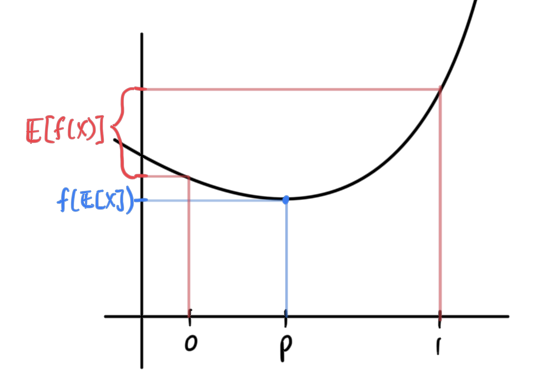
\includegraphics[scale=0.4]{img/jensen_visual.png}
		\caption{The function $f$ essentially transforms the Bernoulli defined on $0, 1$ to the Bernoulli defined on $f(0), f(1)$. Therefore, $\mathbb{E}[f(X)] \in [f(0), f(1)]$, which lies completely over $f(\mathbb{E}[X])$.} 
		\label{fig:jensen_visual}
	\end{figure}

\subsection{Variance}

  \begin{definition}[Variance]
    \label{def:variance}
    Let $X$ be a \hyperref[def:random-variable]{random variable} and suppose $\mathbb{E}[X] < \infty$. The \textbf{variance} of $X$ is defined 
    \begin{equation}
			\mathrm{Var}[X] = \sigma^2_X \coloneqq \mathbb{E} [ (X - \mathbb{E}[X])^2 ]= \mathbb{E}[X^2] - \mathbb{E}[X]^2
    \end{equation}
    and $\sigma_X = \sqrt{\mathrm{Var}[X]}$ is called the \textbf{standard deviation}. This is a measure of how much the probability distribution deviates from its mean. 
  \end{definition}
	\begin{proof}
		We can use linearity of expectation to write 
    \begin{align*}
      \mathrm{Var}[X] & = \mathbb{E} \big[ X^2 + \mathbb{E}[X]^2 - 2 X \mathbb{E}[X] \big] \\
      & = \mathbb{E}[X^2] + \mathbb{E}[X]^2 - 2 \mathbb{E}[X] \mathbb{E}[X] \\
      & = \mathbb{E}[X^2] - \mathbb{E}[X]^2
    \end{align*}
	\end{proof}

	The second formula is often easier to compute, since it only requires us to compute the expectation of $X$ and $X^2$. Since variance is always nonnegative, we also know that $\mathbb{E}[X^2] \geq \mathbb{E}[X]^2$. The variance is always defined, whether it's finite or $+\infty$. 

  \begin{lemma}[Properties of Variance]
    \label{thm:properties-of-variance}
    Let $X$ and $Y$ be \hyperref[def:random-variable]{random variables} with well-defined variances. 
    \begin{enumerate}
      \item \textit{Translation Invariance}: Given that $X + a$ is a new random variable defined $(X + a)(\omega) = X(\omega) + a$, 
      \begin{equation}
        \mathrm{Var}[X] = \mathrm{Var}[X + a]
      \end{equation}
      \item \textit{Quadratic Scaling}: Given that $aX$ is a new random variable defined $(aX)(\omega) = a\,X(\omega)$, 
      \begin{equation}
        \mathrm{Var}[aX] = a^2 \mathrm{Var}[X]
      \end{equation}
      \item \textit{Zero Variance Characterizes Constants}: The variance of $X$ is $0$ if and only if $X$ is constant \hyperref[mt-def:almost_everywhere]{almost everywhere} on $\Omega$. 
    \end{enumerate}
  \end{lemma}
  \begin{proof}
    (1) By linearity of expectation, $\mathbb{E}[X + a] = \mathbb{E}[X] + a$, so $(X + a) - \mathbb{E}[X + a] = X - \mathbb{E}[X]$ and the variances agree. 

    (2) Similarly $\mathbb{E}[aX] = a \mathbb{E}[X]$, so $\mathrm{Var}[aX] = \mathbb{E}[(aX - a\mathbb{E}[X])^2] = a^2 \, \mathbb{E}[(X - \mathbb{E}[X])^2] = a^2 \mathrm{Var}[X]$. 

    (3) If $X = c$ almost everywhere, then $\mathbb{E}[X] = c$ and $(X - \mathbb{E}[X])^2 = 0$ almost everywhere, so $\mathrm{Var}[X] = 0$. Conversely, let $\mathrm{Var}[X] = 0$. Then, 
    \begin{equation}
      \mathrm{Var}[X] = \int_\Omega (X - \mathbb{E}[X])^2 \, d\mathbb{P} = 0
    \end{equation}
    But by nonnegativity of the integrand, we know that $(X - \mathbb{E}[X])^2 = 0$ with probability $1$, which implies that $X = \mathbb{E}[X]$ with probability $1$. 
  \end{proof}

  From the \hyperref[thm:properties-of-expectation]{properties of expectation} and variance, we can now \textbf{standardize} a \hyperref[def:random-variable]{random variable} $X$. If $X$ is a random variable with mean $\mu = \mathbb{E}[X]$ and variance $\sigma^2 = \Var(X)$, then the random variable 
  \begin{equation}
    Y = \frac{X - \mu}{\sigma}
  \end{equation}
  has mean $\mathbb{E}(Y) = 0$ and variance $\Var(Y) = 1$. 

  \hyperref[thm:markovs-inequality]{Markov's inequality} is very conservative but very general, too. If we make further assumptions about the \hyperref[def:random-variable]{random variable} $X$, we can often make stronger bounds. Chebyshev's inequality assumes a (possibly negative) random variable with finite variance and states that the probability will go down as $1/x^2$. 

  \begin{theorem}[Chebyshev Inequality]
    \label{thm:chebyshev-inequality}
    Given (possibly negative) \hyperref[def:random-variable]{random variable} $X$, if $\mathbb{E}[X] = \mu < +\infty$ and $\Var(X) = \sigma^2 < +\infty$, then for all $\alpha > 0$, 
    \begin{equation}
      \mathbb{P} \big( |X - \mu| > k \sigma \big) \leq \frac{1}{k^2} \iff \mathbb{P}(|X - \mu| > \alpha) \leq \frac{\mathrm{Var}[X]}{\alpha^2}
    \end{equation}
    That is, the probability that $X$ takes a value further than $k$ standard deviations away from $\mu$ goes down by $1/k^2$. Therefore, if $\sigma$ is small, then this bound will be small since there is more concentration in the mean. 
  \end{theorem}
  \begin{proof}
    We apply \hyperref[thm:markovs-inequality]{Markov's inequality} to the non-negative \hyperref[def:random-variable]{random variable} $|X - \mu|$. 
    \begin{equation}
      \mathbb{P}(|X - \mu| > \alpha) = \mathbb{P}(|X - \mu|^2 > \alpha^2) \leq \frac{\mathbb{E}(|X - \mu|^2)}{\alpha^2} = \frac{\mathrm{Var}[X]}{\alpha^2}
    \end{equation}
    since the numerator on the RHS is the definition of variance. 
  \end{proof}

  \hyperref[thm:chebyshev-inequality]{Chebyshev inequality} is just \hyperref[thm:markovs-inequality]{Markov's inequality} applied to $X^2$ (assuming $0$ mean), and often yields a better bound.

  \begin{theorem}[Variance of Bernoulli]
    \label{thm:variance-of-bernoulli}
    If \hyperref[def:indicator-bernoulli-random-variable]{$X \sim \Bernoulli(p)$}, then 
    \begin{equation}
      \mathrm{Var}[X] = p (1 - p)
    \end{equation}
  \end{theorem}
  \begin{proof}
    Since $X \in \{0, 1\}$, $X^2 = X$, so $\mathbb{E}[X^2] = p$, and $\mathrm{Var}[X] = \mathbb{E}[X^2] - \mathbb{E}[X]^2 = p - p^2$. 
  \end{proof}

  \begin{theorem}[Variance of Discrete Uniform]
    \label{thm:variance-of-discrete-uniform}
    If \hyperref[def:uniform-random-variable]{$X \sim \Uniform(\mathcal{X})$} with $\mathcal{X} = \{x_1, \ldots, x_n\} \subset \mathbb{R}$ and $\bar{x} = \frac{1}{n} \sum_i x_i$, then 
    \begin{equation}
      \mathrm{Var}[X] = \frac{1}{n} \sum_{i=1}^n (x_i - \bar{x})^2
    \end{equation}
  \end{theorem}
  \begin{proof}
    By the \hyperref[thm:expectation-of-discrete-uniform]{expectation} $\mathbb{E}[X] = \bar{x}$ and \hyperref[thm:lotus]{LOTUS}, $\mathrm{Var}[X] = \mathbb{E}[(X - \bar{x})^2] = \sum_{i} (x_i - \bar{x})^2 \, \mathbb{P}(X = x_i) = \frac{1}{n} \sum_i (x_i - \bar{x})^2$. 
  \end{proof}

  \begin{theorem}[Variance of Geometric]
    \label{thm:variance-of-geometric}
    If \hyperref[def:geometric-random-variable]{$X \sim \Geometric(p)$}, then 
    \begin{equation}
      \mathrm{Var}[X] = \frac{1 - p}{p^2}
    \end{equation}
  \end{theorem}
  \begin{proof}
    Let $q = 1 - p$. Differentiating the geometric series twice, $\sum_{k \geq 2} k(k-1) q^{k-2} = \frac{2}{(1 - q)^3}$, so by \hyperref[thm:lotus]{LOTUS}, 
    \begin{equation}
      \mathbb{E}[X(X-1)] = \sum_{k=2}^\infty k (k-1) q^{k-1} p = p q \cdot \frac{2}{(1-q)^3} = \frac{2q}{p^2}
    \end{equation}
    Then, with $\mathbb{E}[X] = 1/p$, $\mathrm{Var}[X] = \mathbb{E}[X(X-1)] + \mathbb{E}[X] - \mathbb{E}[X]^2 = \frac{2q}{p^2} + \frac{1}{p} - \frac{1}{p^2} = \frac{1-p}{p^2}$. 
  \end{proof}

  \begin{theorem}[Variance of Binomial]
    \label{thm:variance-of-binomial}
    If \hyperref[def:binomial-random-variable]{$X \sim \Binomial(n, p)$}, then 
    \begin{equation}
      \mathrm{Var}[X] = np(1 - p)
    \end{equation}
  \end{theorem}
  \begin{proof}
    Using $k(k-1) \binom{n}{k} = n(n-1) \binom{n-2}{k-2}$ and the binomial theorem, 
    \begin{equation}
      \mathbb{E}[X(X-1)] = \sum_{k=2}^n k(k-1) \binom{n}{k} p^k (1-p)^{n-k} = n(n-1) p^2 \sum_{k=2}^n \binom{n-2}{k-2} p^{k-2} (1-p)^{(n-2)-(k-2)} = n(n-1)p^2
    \end{equation}
    So $\mathrm{Var}[X] = n(n-1)p^2 + np - (np)^2 = np - np^2 = np(1-p)$. 
  \end{proof}

  \begin{theorem}[Variance of Poisson]
    \label{thm:variance-of-poisson}
    If \hyperref[def:poisson-random-variable]{$X \sim \Poisson(\lambda)$}, then 
    \begin{equation}
      \mathrm{Var}[X] = \lambda
    \end{equation}
  \end{theorem}
  \begin{proof}
    Since $k(k-1)/k! = 1/(k-2)!$ for $k \geq 2$, 
    \begin{equation}
      \mathbb{E}[X(X-1)] = \sum_{k=2}^\infty k(k-1) \frac{e^{-\lambda} \lambda^k}{k!} = \lambda^2 \sum_{k=2}^\infty \frac{e^{-\lambda} \lambda^{k-2}}{(k-2)!} = \lambda^2
    \end{equation}
    So $\mathrm{Var}[X] = \lambda^2 + \lambda - \lambda^2 = \lambda$. 
  \end{proof}

  \begin{theorem}[Variance of Negative Binomial]
    \label{thm:variance-of-negative-binomial}
    If \hyperref[def:negative-binomial-distribution]{$X \sim \NegBinomial(r, p)$}, then 
    \begin{equation}
      \mathrm{Var}[X] = \frac{r p}{(1 - p)^2}
    \end{equation}
  \end{theorem}
  \begin{proof}
    For $k \geq 2$, $k(k-1) \binom{k+r-1}{k} = \frac{(k+r-1)!}{(k-2)! \, (r-1)!} = r(r+1) \binom{k+r-1}{k-2}$. Setting $j = k - 2$ and using $\sum_{j} \binom{j+m-1}{j} x^j = (1-x)^{-m}$ with $m = r + 2$, 
    \begin{equation}
      \mathbb{E}[X(X-1)] = r(r+1) p^2 (1-p)^r \sum_{j=0}^\infty \binom{j+r+1}{j} p^j = \frac{r(r+1) p^2}{(1-p)^2}
    \end{equation}
    So $\mathrm{Var}[X] = \frac{r(r+1)p^2}{(1-p)^2} + \frac{rp}{1-p} - \frac{r^2 p^2}{(1-p)^2} = \frac{r p^2}{(1-p)^2} + \frac{rp}{1-p} = \frac{rp}{(1-p)^2}$. 
  \end{proof}

  \begin{theorem}[Variance of Continuous Uniform]
    \label{thm:variance-of-continuous-uniform}
    If \hyperref[def:uniform-random-variable-2]{$X \sim \Uniform(0, 1)$}, then 
    \begin{equation}
      \mathrm{Var}[X] = \frac{1}{12}
    \end{equation}
    More generally, if $X \sim \Uniform(a, b)$, then $\mathrm{Var}[X] = \frac{(b - a)^2}{12}$. 
  \end{theorem}
  \begin{proof}
    By \hyperref[thm:lotus]{LOTUS}, $\mathbb{E}[X^2] = \int_0^1 x^2 \,dx = \frac{1}{3}$, so $\mathrm{Var}[X] = \frac{1}{3} - \frac{1}{4} = \frac{1}{12}$. For $X = a + (b - a) U$, the \hyperref[thm:properties-of-variance]{properties of variance} give $\mathrm{Var}[X] = (b - a)^2 \mathrm{Var}[U] = \frac{(b-a)^2}{12}$. This is consistent with the fact that if we spread out our measure over a wider interval, then the variance will be bigger. 
  \end{proof}

  \begin{theorem}[Variance of Exponential]
    \label{thm:variance-of-exponential}
    If \hyperref[def:exponential-random-variable]{$X \sim \Exponential(\lambda)$}, then 
    \begin{equation}
      \mathrm{Var}[X] = \frac{1}{\lambda^2}
    \end{equation}
  \end{theorem}
  \begin{proof}
    By \hyperref[thm:lotus]{LOTUS} and $\int_0^\infty x^{s-1} e^{-\lambda x} \,dx = \Gamma(s) / \lambda^s$, $\mathbb{E}[X^2] = \lambda \int_0^\infty x^2 e^{-\lambda x} \,dx = \lambda \cdot \frac{\Gamma(3)}{\lambda^3} = \frac{2}{\lambda^2}$. So $\mathrm{Var}[X] = \frac{2}{\lambda^2} - \frac{1}{\lambda^2} = \frac{1}{\lambda^2}$. This is consistent with the fact that if $\lambda$ is greater, then the PDF is much more concentrated at $0$, making the variance small. 
  \end{proof}

  \begin{theorem}[Variance of Gaussian]
    \label{thm:variance-of-gaussian}
    If \hyperref[def:gaussian-random-variable]{$X \sim \Normal(\mu, \sigma^2)$}, then 
    \begin{equation}
      \mathrm{Var}[X] = \sigma^2
    \end{equation}
  \end{theorem}
  \begin{proof}
    With $\mathbb{E}[X] = \mu$, by \hyperref[thm:lotus]{LOTUS} and the substitution $x = \mu + \sigma z$, $\mathrm{Var}[X] = \int (x - \mu)^2 f_X (x) \,dx = \sigma^2 \int_{-\infty}^\infty z^2 \varphi(z) \,dz$. Integrating by parts with $\varphi^\prime (z) = -z \varphi(z)$, 
    \begin{equation}
      \int_{-\infty}^\infty z^2 \varphi(z) \,dz = \Big[ -z \varphi(z) \Big]_{-\infty}^\infty + \int_{-\infty}^\infty \varphi(z) \,dz = 0 + 1 = 1
    \end{equation}
    and so $\mathrm{Var}[X] = \sigma^2$. 
  \end{proof}

  \begin{theorem}[Variance of Cauchy]
    \label{thm:variance-of-cauchy}
    If $X$ is a \hyperref[def:cauchy-random-variable-standardized]{Cauchy random variable}, then $\mathrm{Var}[X]$ is undefined (in fact $\mathbb{E}[X^2] = +\infty$). 
  \end{theorem}
  \begin{proof}
    The variance requires $\mathbb{E}[X]$, which is \hyperref[thm:expectation-of-cauchy]{undefined}. Moreover, by \hyperref[thm:lotus]{LOTUS}, $\mathbb{E}[X^2] = \int_{-\infty}^\infty \frac{x^2}{\pi (1 + x^2)} \,dx = +\infty$ since the integrand tends to $1/\pi$ as $|x| \to \infty$. 
  \end{proof}

  \begin{theorem}[Variance of Gamma]
    \label{thm:variance-of-gamma}
    If \hyperref[def:gamma-random-variable]{$X \sim \GammaDist(\alpha, \beta)$}, then 
    \begin{equation}
      \mathrm{Var}[X] = \frac{\alpha}{\beta^2}
    \end{equation}
  \end{theorem}
  \begin{proof}
    By \hyperref[thm:lotus]{LOTUS} and $\int_0^\infty x^{s-1} e^{-\beta x} \,dx = \Gamma(s) / \beta^s$, $\mathbb{E}[X^2] = \frac{\beta^\alpha}{\Gamma(\alpha)} \cdot \frac{\Gamma(\alpha + 2)}{\beta^{\alpha + 2}} = \frac{\alpha (\alpha + 1)}{\beta^2}$. So $\mathrm{Var}[X] = \frac{\alpha(\alpha+1)}{\beta^2} - \frac{\alpha^2}{\beta^2} = \frac{\alpha}{\beta^2}$. 
  \end{proof}

  \begin{theorem}[Variance of Beta]
    \label{thm:variance-of-beta}
    If \hyperref[def:beta-random-variable]{$X \sim \BetaDist(\alpha, \beta)$}, then 
    \begin{equation}
      \mathrm{Var}[X] = \frac{\alpha \beta}{(\alpha + \beta)^2 (\alpha + \beta + 1)}
    \end{equation}
  \end{theorem}
  \begin{proof}
    By \hyperref[thm:lotus]{LOTUS}, $\mathbb{E}[X^2] = \frac{B(\alpha + 2, \beta)}{B(\alpha, \beta)} = \frac{\alpha (\alpha + 1)}{(\alpha + \beta)(\alpha + \beta + 1)}$. So 
    \begin{equation}
      \mathrm{Var}[X] = \frac{\alpha (\alpha + 1)}{(\alpha + \beta)(\alpha + \beta + 1)} - \frac{\alpha^2}{(\alpha + \beta)^2} = \frac{\alpha \big[ (\alpha + 1)(\alpha + \beta) - \alpha (\alpha + \beta + 1) \big]}{(\alpha + \beta)^2 (\alpha + \beta + 1)} = \frac{\alpha \beta}{(\alpha + \beta)^2 (\alpha + \beta + 1)}
    \end{equation}
  \end{proof}

  Just like how we explained that computing finiteness or infiniteness of expectation is similar to multiplying the PMF/PDF by $x$ and determining if the series/integral converges or diverges, we can do the same for variance by multiplying the PMF/PDF by $x^2$. For a probability distribution of form $\frac{1}{x^2}$, it diverges if we multiply by $x$ and also diverges if we multiply by $x^2$. But also, we could construct a distribution where the expectation may be finite, but the variance may be infinite. For example, if we have a distribution of form $\frac{1}{x^3}$, multiplying it by $x$ leads to form $\frac{1}{x^2}$, which is finite (so finite expectation), but multiplying by $x^2$ leads to a harmonic, i.e. infinite variance. 

\subsection{Higher Moments} 

  \begin{definition}[Moment]
    \label{def:moment}
    The \textbf{$\mathbf{n}$th (raw) moment} of a \hyperref[def:random-variable]{random variable} $X$ is $\mathbb{E}[X^n]$. Unlike the raw moment, which is calculated around the origin, the \textbf{$\mathbf{n}$th central moment} of $X$ is its moment centered around its mean $\mathbb{E}[(X - \mathbb{E}[X])^n]$. 
    \begin{enumerate}
      \item the first moment is the mean $\mathbb{E}[X]$
      \item the second central moment is the variance $\mathbb{E}[(X - \mathbb{E}[X])^2]$ 
      \item the third central moment, divided by $\sigma^3$, is the skew $\frac{1}{\sigma^3} \mathbb{E}[(X - \mathbb{E}[X])^3]$ 
    \end{enumerate}
  \end{definition}

  \begin{definition}[Convergence in rth Mean]
    \label{def:convergence-in-rth-mean}
    We say $X_n$ \textbf{converges to $X$ in the $r$th mean} if 
    \begin{equation}
      \lim_{n \rightarrow \infty} \mathbb{E} \big[ |X_n - X|^r \big] = 0
    \end{equation}
    For $r = 2$, $X_n$ is said to converge to $X$ in the \textbf{mean-squared sense}. 
  \end{definition}

  \begin{theorem}[Convergence in $r$th Mean Implies Convergence in Probability]
    \label{thm:rth-mean-implies-in-probability}
    If $X_n \to X$ in the $r$th mean, then $X_n \xrightarrow{i.p.} X$ (and therefore also in distribution, by the \hyperref[thm:hierarchy-of-convergence]{hierarchy of convergence}). 
  \end{theorem}
  \begin{proof}
    For any $\epsilon > 0$, by \hyperref[thm:markovs-inequality]{Markov's inequality} applied to the non-negative random variable $|X_n - X|^r$, 
    \begin{equation}
      \mathbb{P}(|X_n - X| > \epsilon) = \mathbb{P}(|X_n - X|^r > \epsilon^r) \leq \frac{\mathbb{E}[|X_n - X|^r]}{\epsilon^r} \to 0
    \end{equation}
  \end{proof}

\subsection{Covariance and Correlation}

  The variance is a measure for one \hyperref[def:random-variable]{random variable} $X$, which measures how much it deviates from its mean. Now, the covariance is defined for two random variables and captures how they jointly vary. 

  \begin{definition}[Covariance]
    \label{def:covariance}
    The \textbf{covariance} of \hyperref[def:random-variable]{random variables} $X$ and $Y$ is defined as 
    \begin{align*}
      \mathrm{Cov}[X, Y] & = \mathbb{E} \big[ (X - \mathbb{E}[X]) (Y - \mathbb{E}[X]) \big] \\
      & = \mathbb{E}[X Y] - \mathbb{E}[X] \, \mathbb{E}[Y]
    \end{align*}
    where the intermediate expectations are well-defined. $X$ and $Y$ are said to be \textbf{uncorrelated} if 
    \begin{equation}
      \mathrm{Cov}[X, Y] = 0
    \end{equation}
  \end{definition}

  The covariance is also easy to interpret. Given two \hyperref[def:random-variable]{random variables} $X$ and $Y$, if whenever $X$ is greater than its expected value $\mathbb{E}[X]$, $Y$ also tends to be greater than $\mathbb{E}[Y]$, then the covariance will be some positive number. If they tend to be on opposite sides of their expected values, then the covariance will be negative. And the degree with which these RVs lie on which side of the expected value determines the magnitude of the covariance. 

  \begin{theorem}[Independence Implies Uncorrelatedness]
    \label{thm:independence-implies-uncorrelatedness}
    If $X$ and $Y$ are \hyperref[def:independent-random-variables]{independent random variables}, then they are uncorrelated, meaning that independence is a stronger condition. 
  \end{theorem}

  We show an example of why the converse is not true. Consider $X \sim \Uniform[-1, 1]$. We can show that $x$ and $Y = X^2$ are dependent but uncorrelated. It is clearly dependent, but its covariance is 
  \begin{align*}
    \mathrm{Cov}(X, Y) & = \mathbb{E}[X Y] - \mathbb{E}[X] \, \mathbb{E}[Y] \\
    & = \mathbb{E}[X^3] - \mathbb{E}[X] \, \mathbb{E}[X^2] \\
    & = \int_{-1}^1 x^3 \cdot 1 \,dx - 0 \cdot \mathbb{E}[X^2] = 0
  \end{align*}

  \begin{definition}[Multivariate Gaussian]
    \label{def:multivariate-gaussian}
		Let us have a vector-valued \hyperref[def:random-variable]{random variable} $\mathbf{X} = (X_1 \ldots X_n)^T \sim \mathcal{N}(\boldsymbol{\mu}, \boldsymbol{\Sigma})$. 
		\begin{enumerate}
			\item $\mathbf{X}$ is a \textbf{multivariate Gaussian distribution} with mean $\boldsymbol{\mu} \in \mathbb{R}^n$ and symmetric, positive-definite covariance matrix $\boldsymbol{\Sigma} \in \mathbb{R}^{n \times n}$ if its probability density function is
			\begin{equation}
			  f_X (x) = \frac{1}{(2\pi)^{n/2} \mathrm{det}(\boldsymbol{\Sigma})^{1/2}} \exp\bigg( -\frac{1}{2} (x-\boldsymbol{\mu})^T \boldsymbol{\Sigma}^{-1} (x - \boldsymbol{\mu})\bigg)
			\end{equation}
			The covariance matrix $\boldsymbol{\Sigma}$ is the $n \times n$ matrix whose $(i, j)$th entry is $\Cov(X_i, X_j)$. That is, for any random vector $\mathbf{X}$ with mean $\boldsymbol{\mu}$, its covariance matrix 
			\begin{equation}
			  \boldsymbol{\Sigma} = \mathbb{E}\big[ (\mathbf{X} - \boldsymbol{\mu}) (\mathbf{X} - \boldsymbol{\mu})^T \big] = \mathbb{E}[\mathbf{X} \mathbf{X}^T] - \boldsymbol{\mu} \boldsymbol{\mu}^T
			\end{equation}
			is positive definite and symmetric, which implies by the spectral theorem we can break it down into $n$ orthogonal eigenspaces of positive eigenvalues. 

			\item $X$ is a multivariate Gaussian distribution if it can be expressed as 
			\begin{equation}
			  \mathbf{X} = \mathbf{D} \mathbf{w} + \boldsymbol{\mu}
			\end{equation}
			where $\mathbf{w}$ is a vector of independent $\mathcal{N}(0, 1)$ Gaussians, $\boldsymbol{\mu} \in \mathbb{R}^n$, and $\mathbf{D} \in \mathbb{R}^{n \times n}$. The mean of $\mathbf{X}$ is $\boldsymbol{\mu}$ and its covariance is $\boldsymbol{\Sigma} = \mathbf{D} \mathbf{D}^T$; $\mathbf{D}$ is called the \textbf{standard deviation matrix}. When modeling high-dimensional Gaussians, this way is most computationally feasible. 

			\item $X$ is a multivariate Gaussian distribution if for every $\mathbf{a} \in \mathbb{R}^n$, $\mathbf{a}^T \mathbf{x}$ is a Gaussian RV. This means that if we take $\mathbf{a} = \mathbf{0}$, then the entire $\mathbf{X}$ is constantly $0$, which we will take to be the degenerate Gaussian with mean, variance $0$. 
		\end{enumerate}
		The $n$ semi-axes of the $(n-1)$-dimensional isocontour ellipsoid formed by an $n$-dimensional Gaussian distribution are precisely the normalized eigenvectors of $\boldsymbol{\Sigma}$ multiplied by their eigenvalues. 
  \end{definition}

  If we let $\boldsymbol{\Sigma} = \mathbf{I}$, then this means that all the $X_i$'s are pairwise uncorrelated since $\Sigma_{ij} = \Cov (X_i, X_j) = 0$. In general, this does not mean that the $X_i$'s are independent, but for joint Gaussians, this also implies independence! 

	\begin{theorem}[Uncorrelated Equals Independence in Multivariate Gaussian]
	  \label{thm:uncorrelated-equals-independence-in}
		Given \hyperref[def:multivariate-gaussian]{multivariate Gaussian} $\mathbf{X} = (X_1 \ldots X_n)^T \sim \mathcal{N}(\boldsymbol{\mu}, \boldsymbol{\Sigma})$, the $X_i$'s are pairwise independent if and only if they are uncorrelated. 
  \end{theorem}
  \begin{proof}
		We can expand the PDF of $\mathbf{X}$ as 
		\begin{align}
			f_X (x) & = \frac{1}{(2 \pi)^{n/2}} \exp \bigg( -\frac{1}{2} (x - \mu)^T (x - \mu) \bigg) \\
			& = \bigg(\frac{1}{\sqrt{2\pi}} \bigg)^n \exp \bigg( \sum_{i=1}^n -\frac{1}{2} (x_i - \mu_i)^2 \bigg) \\
			& = \prod_{i=1}^n \frac{1}{\sqrt{2\pi}} \exp \bigg( -\frac{1}{2} (x_i - \mu_i)^2 \bigg)
		\end{align}
		which is the product of $n$ single-variable Gaussians $X_i$. Therefore this means that independence and uncorrelation are equivalent! 
  \end{proof}

  \begin{theorem}[Variance of Sums of Random Variables]
    \label{thm:variance-of-sums-of-random-variables}
    If $X$ and $Y$ are two \hyperref[def:random-variable]{random variables}, then 
    \begin{equation}
      \mathrm{Var}(X + Y) = \mathrm{Var}[X] + \mathrm{Var}(Y) + 2 \mathrm{Cov}(X, Y)
    \end{equation}
    and by induction, we can show that 
    \begin{equation}
      \mathrm{Var}\bigg( \sum_i X_i\bigg) = \sum_{i} \mathrm{Var}(X_i) + \sum_{i, j} \mathrm{Cov}(X_i, X_j)
    \end{equation}
  \end{theorem}
  \begin{proof}
    Simple computation. The LHS expands to 
    \begin{align*}
      \mathbb{E}[(X + Y)^2] - \mathbb{E}[X + Y]^2 & = \mathbb{E}[X^2 + 2XY + Y^2] - (\mathbb{E}[X] + \mathbb{E}[Y])^2 \\
      & = \mathbb{E}[X^2] + 2 \mathbb{E}[XY] + \mathbb{E}[Y^2] - \mathbb{E}[X]^2 - 2 \mathbb{E}[X] \mathbb{E}[Y] - \mathbb{E}[Y]^2 \\
      & = \big( \mathbb{E}[X^2] - \mathbb{E}[X]^2 \big) + \big( \mathbb{E}[Y^2] - \mathbb{E}[Y]^2 \big) + 2 \big( \mathbb{E}[XY] - \mathbb{E}[X] \mathbb{E}[Y] \big) \\
      & = \mathrm{Var}[X] + \mathrm{Var}(Y) + 2 \mathrm{Cov}(X, Y) 
    \end{align*}
  \end{proof}

  Therefore, if we have $n$ \hyperref[def:random-variable]{random variables} $X_1, \ldots, X_n$, then we can compute their pairwise covariance $\mathrm{Cov}(X_i, X_j)$ and compute their \textbf{covariance matrix} $\boldsymbol{\Sigma}$, which is an $n \times n$ symmetric matrix with entries 
  \begin{equation}
    \boldsymbol{\Sigma}_{ij} = \mathrm{Cov}(X_i, X_j) \text{ for } i, j = 1, \ldots, n
  \end{equation}

  \begin{theorem}[Simple Bound on Covariance]
    \label{thm:simple-bound-on-covariance}
    If $X$ and $Y$ are two \hyperref[def:random-variable]{random variables} with finite variance, then the magnitude of their covariance is bounded by the following inequality. 
    \begin{equation}
      |\Cov(X,Y)| \leq \sqrt{\Var(X) \, \Var(Y)} = \std(X) \, \std(Y)
    \end{equation}
  \end{theorem}

  Finally we define the correlation. 

  \begin{definition}[Correlation Coefficient]
    \label{def:correlation-coefficient}
    The \textbf{correlation coefficient} of \hyperref[def:random-variable]{random variables} $X$ and $Y$ is defined 
    \begin{equation}
      \rho_{X, Y} = \mathrm{Corr}(X, Y) \coloneqq \frac{\mathrm{Cov}(X, Y)}{\sigma_X \sigma_Y} = \frac{\mathrm{Cov}(X, Y)}{\sqrt{\mathrm{Var}[X] \, \mathrm{Var}(Y)}}
    \end{equation}
  \end{definition}

  By definition, this implies that $-1 \leq \Corr(X, Y) \leq 1$. When $\Corr(X, Y) > 0$ (which also means that $\Cov(X, Y) > 0$), it is said that $X$ and $Y$ are \textit{positively correlated}, and when $\Corr(X, Y) < 0$ (which also means that $\Cov(X, Y) < 0$), it is said that they are \textit{negatively correlated}. 

  \begin{theorem}[Correlation $\pm 1$ Characterizes Linear Dependence]
    \label{thm:correlation-pm1-characterizes-linear-dependence}
    $\Corr(X,Y) = \pm 1$ indicates a linear relationship between $X$ and $Y$. 
    \begin{enumerate}
      \item Let $\Corr(X, Y) = 1$. Then, there exists a $m>0$ and $b \in \mathbb{R}$ such that $Y = m X + b$. 
      \item Let $\Corr(X, Y) = -1$. Then, there exists a $m<0$ and $b \in \mathbb{R}$ such tat $Y = m X + b$. 
    \end{enumerate}
    This implies that $\Corr(X, Y) = \pm 1$ indicates that the joint distribution of $(X, Y)$ is concentrated on a line in $\mathbb{R}^2$. 
  \end{theorem}

  In some sense the correlation is a scaled version of the covariance. It is scale-invariant, and it is always a number that lies between $-1$ and $1$, making it a nice way to represent the correlation between two variables without having to worry about scale. We can prove this. 

  \begin{theorem}[Marginals of a Standard Bivariate Gaussian]
    \label{thm:marginals-of-a-standard-bivariate-gaussian}
    Let $(X, Y) \sim \mathcal{N}(\mathbf{0}, \boldsymbol{\Sigma})$ be a \hyperref[def:multivariate-gaussian]{standard bivariate Gaussian} with $\boldsymbol{\Sigma} = \begin{pmatrix} 1 & \rho \\ \rho & 1 \end{pmatrix}$ and $|\rho| < 1$, so that its joint PDF is 
    \begin{equation}
      f_{X, Y} (x, y) = \frac{1}{2 \pi \sqrt{1 - \rho^2}} \exp \bigg( -\frac{x^2 - 2 \rho x y + y^2}{2 (1 - \rho^2)}\bigg)
    \end{equation}
    Then, 
    \begin{enumerate}
      \item $X$ and $Y$ are marginally distributed as $\mathcal{N}(0, 1)$. That is, if we integrate a variable (say, $x$) out, we will get a univariate standard Gaussian PDF of the other ($y$): 
      \begin{equation}
        \int_{-\infty}^\infty \frac{1}{2 \pi \sqrt{1 - \rho^2}} \exp \bigg( -\frac{x^2 - 2 \rho x y + y^2}{2 (1 - \rho^2)}\bigg) \,dx = \frac{1}{\sqrt{2 \pi}} e^{-y^2 / 2}
      \end{equation}
      \item $\rho_{X, Y}$, the \hyperref[def:correlation-coefficient]{correlation coefficient} of $X$ and $Y$, is equal to $\rho$. 
    \end{enumerate}
  \end{theorem}
  \begin{proof}
    (1) Completing the square in $x$, $x^2 - 2 \rho x y + y^2 = (x - \rho y)^2 + (1 - \rho^2) y^2$, so 
    \begin{equation}
      \int_{-\infty}^\infty f_{X, Y} (x, y) \,dx = \frac{e^{-y^2/2}}{2 \pi \sqrt{1 - \rho^2}} \int_{-\infty}^\infty \exp \bigg( -\frac{(x - \rho y)^2}{2 (1 - \rho^2)} \bigg) \,dx = \frac{e^{-y^2/2}}{2 \pi \sqrt{1 - \rho^2}} \sqrt{2 \pi (1 - \rho^2)} = \frac{e^{-y^2/2}}{\sqrt{2 \pi}}
    \end{equation}
    and $X$ is symmetric. 

    (2) By the definition of the covariance matrix, $\Cov(X, Y) = \Sigma_{12} = \rho$ and $\Var(X) = \Var(Y) = 1$, so $\rho_{X, Y} = \Cov(X, Y) / \sqrt{\Var(X) \Var(Y)} = \rho$. 
  \end{proof}

  The formula of the general bivariate Gaussian $\mathbf{X} = (X_1, X_2)$ PDF is messy, but we will put it here. 
	\begin{align}
		f_{X_1, X_2} (x_1 , x_2) & = \frac{1}{2 \pi \sqrt{\mathrm{det}(\boldsymbol{\Sigma})}} \exp \bigg( - \frac{(\mathbf{x} - \boldsymbol{\mu})^T \boldsymbol{\Sigma}^{-1} (\mathbf{x} - \boldsymbol{\mu})}{2} \bigg) \\ 
														 & = \frac{1}{2 \pi \sigma_1 \sigma_2 \sqrt{1 - \rho^2}} \exp \bigg[ -\frac{1}{2} \bigg( \frac{(x_1 - \mu_1)^2}{\sigma_1^2} + \frac{(x_2 - \mu_2)^2}{\sigma_2^2} - 2 \rho \frac{(x_1 - \mu_1)}{\sigma_1} \frac{(x_2 - \mu_2)}{\sigma_2}\bigg)\bigg]
	\end{align}
  It is cleaner to put it into matrix form. 
  where 
  \begin{equation}
    \mathbf{x} = \begin{pmatrix} x_1 \\ x_2 \end{pmatrix}, \;\; \boldsymbol{\mu} = \begin{pmatrix} \mu_1 \\ \mu_2 \end{pmatrix} , \;\; \boldsymbol{\Sigma} = \mathbb{E}\big[ (\mathbf{X} - \boldsymbol{\mu}) (\mathbf{X} - \boldsymbol{\mu})^T \big] = \begin{pmatrix} \mathrm{Var}(X_1) & \mathrm{Cov}(X_1, X_2) \\
      \mathrm{Cov}(X_1, X_2) & \mathrm{Var}(X_2) \end{pmatrix}
  \end{equation}

  Note that visually, $\boldsymbol{\Sigma}$ will determine how much the Gaussian distribution is "stretched" on one way or another. Obviously, the "peak" of the distribution will be $\boldsymbol{\mu}$. 

	\begin{figure}[H]
		\centering 
		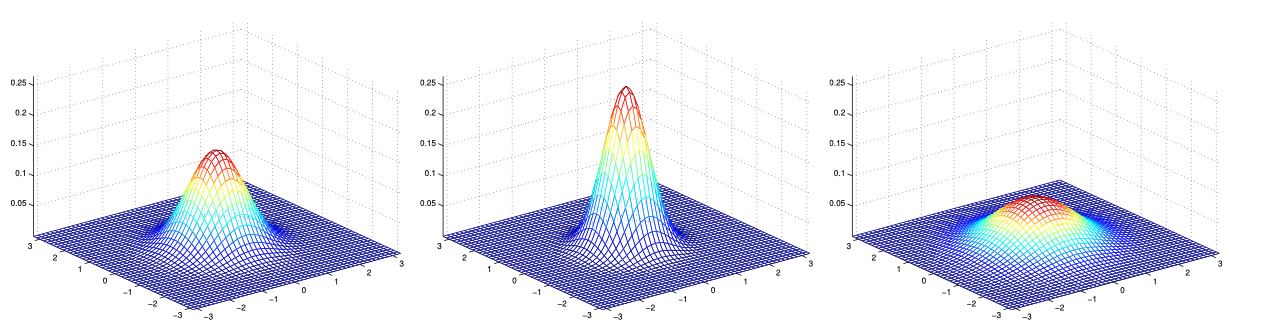
\includegraphics[scale=0.65]{img/Gaussian_Distribution.png}
		\caption{If $\boldsymbol{\Sigma} = I$, then we could visualize the Gaussian distribution as being perfectly symmetric. However, if we scale the distribution up to a certain constant (shown for $\boldsymbol{\Sigma} = I$, $\boldsymbol{\Sigma} = 0.61 I$, $\boldsymbol{\Sigma} = 2 I$), we get the following.} 
		\label{fig:bivariate_gaussian}
	\end{figure}

  \begin{theorem}[Cauchy-Schwarz]
    \label{thm:cauchy-schwarz}
    For any two \hyperref[def:random-variable]{random variables} $X, Y$, we have $|\mathrm{Cov}(X, Y)| \leq \sigma_X \sigma_Y$, or in other words, 
    \begin{equation}
      -1 \leq \rho_{X, Y} \leq 1
    \end{equation}
    Furthermore, whenever $\rho_{X, Y} = 1$ or $-1$, there exists a deterministic relationship between $X$ and $Y$. 
    \begin{enumerate}
      \item If $\rho_{X, Y} = 1$, there exists a $a > 0$ s.t. 
      \begin{equation}
        Y - \mathbb{E}[Y] = a (X - \mathbb{E}[X])
      \end{equation}
      \item If $\rho_{X, Y} = -1$ there exists a $a < 0$ s.t. 
      \begin{equation}
        Y - \mathbb{E}[Y] = a (X - \mathbb{E}[X])
      \end{equation}
    \end{enumerate}
    This implies that $\Corr(X, Y) = \pm 1$ indicates that the joint distribution of $(X, Y)$ is concentrated on a line in $\mathbb{R}^2$. 
  \end{theorem}

  The fact that this is called the \hyperref[mt-thm:cauchy-schwarz]{Cauchy-Schwarz} inequality hints at the existence of \hyperref[lin-def:inner-product]{inner products}, norms, and \hyperref[lin-def:vector-space]{vector spaces}. That is, we can treat the \hyperref[def:random-variable]{random variables} $X, Y$ as vectors in the functional space of real-valued maps over $\Omega$. In some sense, $\mathrm{Cov}(X, Y)$ sort-of plays the role of an inner product. 
  \begin{enumerate}
    \item It satisfies symmetricity: 
    \begin{equation}
      \mathrm{Cov}(X, Y) = \mathbb{E}[X Y] - \mathbb{E}[X] \, \mathbb{E}[Y] =  \mathbb{E}[Y X] - \mathbb{E}[Y] \, \mathbb{E}[X] = \mathrm{Cov}(Y, X)
    \end{equation}
    
    \item It satisfies binlinearity. It suffices to show only for first argument, since we have symmetricity. 
    \begin{align*}
      \mathrm{Cov}(aX + bY, Z) & = \mathbb{E}[(a X + b Y) Z] - \mathbb{E}[a X + b Y] \, \mathbb{E}[Z] \\
      & = a \mathbb{E}[X Z] + b \mathbb{E}[Y Z] - a \mathbb{E}[X] \mathbb{E}[Z] - b \mathbb{E}[Y] \, \mathbb{E}[Z] \\
      & = a \big( \mathbb{E}[X Z] - \mathbb{E}[X] \mathbb{E}[Z] \big) + a \big( \mathbb{E}[Y Z] - \mathbb{E}[Y] \, \mathbb{E}[Z] \big) \\
      & = a \, \mathrm{Cov}(X, Z) + b \, \mathrm{Cov}(Y, Z)
    \end{align*}

    \item We want the inner product of $X$ with itself to always be greater than $0$, with equality holding iff $X = 0$. Indeed, we have 
    \begin{equation}
      \mathrm{Cov}(X, X) = \mathrm{Var}[X] \geq 0
    \end{equation}
    but it is not necessarily true that $\mathrm{Var}[X] = 0 \implies X = 0$. We can say that $X$ is equal to a constant \hyperref[mt-def:almost_everywhere]{almost everywhere} at best. We can solve this problem by looking at the functional subspace of $0$-mean random variables (which is a vector space due to linearity of expectation). So now all random variables $X$ that are $0$ almost everywhere have inner product $0$, so we must add an equivalence class on this subspace that says two $X, Y$ are equivalent if they agree almost everywhere. 
  \end{enumerate}

  The standard deviation $\sigma_X$ and $\sigma_Y$ act as norms on this quotient subspace of $0$-mean random variables. So the \hyperref[def:correlation-coefficient]{correlation coefficient} $\rho_{X, Y}$ can be interpreted as the cosine of the angle between $X$ and $Y$. This now makes our desired space a \hyperref[fa-def:hilbert-space]{Hilbert space}, and our uncorrelated random variables are like \hyperref[lin-def:orthogonal-vectors]{orthogonal vectors}. 

  \begin{definition}[The Hilbert Space $L^2_\mathcal{F}(\Omega)$]
    \label{def:the-hilbert-space-l2fomega}
    Let $L^2_\mathcal{F} (\Omega)$ be the function space consisting of equivalence classes of $0$-mean \hyperref[def:random-variable]{random variables} $X: (\Omega, \mathcal{F}) \rightarrow \mathbb{R}$ that are almost surely equal. Then, 
    \begin{enumerate}
      \item we can define the \hyperref[lin-def:inner-product]{inner product} on this space as 
      \begin{equation}
        \langle X, Y \rangle \coloneqq \mathbb{E}[X Y] - \mathbb{E}[X] \mathbb{E}[Y] = \mathbb{E}[X Y] = \int_\Omega X Y \,d\mathbb{P}
      \end{equation}

      \item which induces the $L^2$-norm on this space defined 
      \begin{equation}
        \|X\|_2 \coloneqq \mathrm{Var}(X) = \mathbb{E}[X^2] - \mathbb{E}[X]^2 = \mathbb{E}[X^2] = \int_\Omega X^2 \,d\mathbb{P}
      \end{equation}
    \end{enumerate}
    We set $L^2_\mathcal{F} (\Omega)$ to be a \hyperref[mv-def:banach-space]{Banach space} with bounded norm $\mathbb{E}[X^2] < \infty$. 
  \end{definition}

  Viewing the covariance as an \hyperref[lin-def:inner-product]{inner product} lets us state a remarkable property of the Gaussian: taking the covariance of a Gaussian against a function of itself is the same as differentiating that function. This is a consequence of the fact that the standard Gaussian density $\varphi$ satisfies the differential equation $\varphi^\prime (z) = - z \varphi(z)$, so that multiplication by $z$ inside a Gaussian integral can always be traded for a derivative. 

  \begin{lemma}[Gaussian Integration by Parts]
    \label{thm:gaussian-ibp}
    Let $X \sim \mathcal{N}(\mu, \sigma^2)$ and let $f: \mathbb{R} \rightarrow \mathbb{R}$ be absolutely continuous with $\mathbb{E}|f^\prime (X)| < \infty$. Then 
    \begin{equation}
      \Cov \big( X, f(X) \big) = \sigma^2 \, \mathbb{E}[f^\prime (X)]
    \end{equation}
    In particular, if $Z \sim \mathcal{N}(0, 1)$, then $\mathbb{E}[Z f(Z)] = \mathbb{E}[f^\prime (Z)]$. 

    More generally, let $X = (X_1 \ldots X_n)^T \sim \mathcal{N}(\mu, \Sigma)$ and let $F: \mathbb{R}^n \rightarrow \mathbb{R}$ be differentiable with $\mathbb{E}| \partial_j F (X)| < \infty$ for every $j$. Then for each $i$, 
    \begin{equation}
      \Cov \big( X_i, F(X) \big) = \sum_{j=1}^n \Sigma_{ij} \, \mathbb{E} \big[ \partial_j F (X) \big] 
    \end{equation}
    or in vector form, $\Cov \big( X, F(X) \big) = \Sigma \, \mathbb{E}[\nabla F (X)]$. 
  \end{lemma}
  \begin{proof}
    We first prove the standard univariate case $Z \sim \mathcal{N}(0, 1)$, with density $\varphi(z) = e^{-z^2/2} / \sqrt{2\pi}$. Since $\varphi^\prime (t) = -t \varphi(t)$ and $\varphi$ vanishes at $\pm \infty$, we can write the density itself as a tail integral 
    \begin{equation}
      \varphi(z) = \int_z^\infty t \varphi(t) \,dt \text{ for } z \geq 0, \;\;\;\;\; \varphi(z) = \int_{-\infty}^z (-t) \varphi(t) \,dt \text{ for } z < 0
    \end{equation}
    Substituting these into $\mathbb{E}[f^\prime (Z)]$ and applying Fubini (justified by $\mathbb{E}|f^\prime (Z)| < \infty$) to swap the order of integration, we have on the positive half-line 
    \begin{align*}
      \int_0^\infty f^\prime (z) \varphi(z) \,dz & = \int_0^\infty f^\prime (z) \int_z^\infty t \varphi(t) \,dt \,dz \\
      & = \int_0^\infty t \varphi(t) \int_0^t f^\prime (z) \,dz \,dt \\
      & = \int_0^\infty t \varphi(t) \big( f(t) - f(0) \big) \,dt
    \end{align*}
    and symmetrically on the negative half-line 
    \begin{align*}
      \int_{-\infty}^0 f^\prime (z) \varphi(z) \,dz & = \int_{-\infty}^0 f^\prime (z) \int_{-\infty}^z (-t) \varphi(t) \,dt \,dz \\
      & = \int_{-\infty}^0 (-t) \varphi(t) \int_t^0 f^\prime (z) \,dz \,dt \\
      & = \int_{-\infty}^0 t \varphi(t) \big( f(t) - f(0) \big) \,dt
    \end{align*}
    Adding the two halves and using $\mathbb{E}[Z] = 0$ gives 
    \begin{equation}
      \mathbb{E}[f^\prime (Z)] = \int_{-\infty}^\infty t \varphi(t) \big( f(t) - f(0) \big) \,dt = \mathbb{E}[Z f(Z)] - f(0) \, \mathbb{E}[Z] = \mathbb{E}[Z f(Z)]
    \end{equation}
    For general $X \sim \mathcal{N}(\mu, \sigma^2)$, write $X = \mu + \sigma Z$ and set $g(z) \coloneqq f(\mu + \sigma z)$, so that $g^\prime (z) = \sigma f^\prime (\mu + \sigma z)$. By bilinearity of the covariance and the fact that a constant has $0$ covariance with anything, 
    \begin{align*}
      \Cov \big( X, f(X) \big) & = \Cov \big( \mu + \sigma Z, g(Z) \big) = \sigma \, \Cov \big( Z, g(Z) \big) \\
      & = \sigma \, \mathbb{E}[Z g(Z)] = \sigma \, \mathbb{E}[g^\prime (Z)] = \sigma^2 \, \mathbb{E}[f^\prime (X)]
    \end{align*}
    where $\Cov(Z, g(Z)) = \mathbb{E}[Z g(Z)]$ since $\mathbb{E}[Z] = 0$. 

    For the multivariate case, write $X = \mu + A W$ where $W = (W_1 \ldots W_n)^T$ has iid $\mathcal{N}(0, 1)$ components and $A A^T = \Sigma$. Setting $G(w) \coloneqq F(\mu + A w)$, the \hyperref[mv-thm:chain-rule]{chain rule} gives $\partial_k G (w) = \sum_{j} A_{jk} \, \partial_j F (\mu + A w)$. Since $W_k$ is independent of the remaining coordinates $W_{-k}$, we can condition on $W_{-k}$ and apply the univariate result to the single variable $W_k$, 
    \begin{equation}
      \mathbb{E}[W_k \, G(W)] = \mathbb{E} \big[ \mathbb{E}[ W_k \, G(W) \mid W_{-k} ] \big] = \mathbb{E} \big[ \mathbb{E}[ \partial_k G(W) \mid W_{-k}] \big] = \mathbb{E}[\partial_k G(W)]
    \end{equation}
    Therefore, expanding $X_i = \mu_i + \sum_k A_{ik} W_k$ and using bilinearity again, 
    \begin{align*}
      \Cov \big( X_i, F(X) \big) & = \sum_{k=1}^n A_{ik} \, \Cov \big( W_k, G(W) \big) = \sum_{k=1}^n A_{ik} \, \mathbb{E}[\partial_k G(W)] \\
      & = \sum_{k=1}^n \sum_{j=1}^n A_{ik} A_{jk} \, \mathbb{E} \big[ \partial_j F(X) \big] \\
      & = \sum_{j=1}^n (A A^T)_{ij} \, \mathbb{E} \big[ \partial_j F(X) \big] = \sum_{j=1}^n \Sigma_{ij} \, \mathbb{E} \big[ \partial_j F(X) \big]
    \end{align*}
  \end{proof}

\subsection{Exercises}

  \begin{exercise}[Durrett 1.3.1]
    Show that if $\mathcal{A}$ generates $\mathcal{S}$, then $X^{-1}(\mathcal{A}) \coloneqq \{\{X \in A\} : A \in \mathcal{A}\}$ generates $\sigma(X) = \{\{X \in B\} : B \in \mathcal{S}\}$.
  \end{exercise}
  \begin{solution}

  \end{solution}

  \begin{exercise}[Durrett 1.3.2]
    Prove Theorem 1.3.6 when $n = 2$ by checking $\{X_1 + X_2 < x\} \in \mathcal{F}$.
  \end{exercise}
  \begin{solution}

  \end{solution}

  \begin{exercise}[Durrett 1.3.3]
    Show that if $f$ is continuous and $X_n \to X$ almost surely then $f(X_n) \to f(X)$ almost surely.
  \end{exercise}
  \begin{solution}

  \end{solution}

  \begin{exercise}[Durrett 1.3.4]
    \begin{enumerate}
      \item Show that a \hyperref[pst-def:continuous_func]{continuous function} from $\mathbf{R}^d \to \mathbf{R}$ is a measurable map from $(\mathbf{R}^d, \mathcal{R}^d)$ to $(\mathbf{R}, \mathcal{R})$.
      \item Show that $\mathcal{R}^d$ is the smallest $\sigma$-field that makes all the continuous functions measurable.
    \end{enumerate}
  \end{exercise}
  \begin{solution}

  \end{solution}

  \begin{exercise}[Durrett 1.3.5]
    A function $f$ is said to be \textbf{lower semicontinuous} or l.s.c. if
    \begin{equation*}
      \liminf_{y \to x} f(y) \geq f(x)
    \end{equation*}
    and \textbf{upper semicontinuous} (u.s.c.) if $-f$ is l.s.c. Show that $f$ is l.s.c. if and only if $\{x : f(x) \leq a\}$ is closed for each $a \in \mathbf{R}$ and conclude that semicontinuous functions are measurable.
  \end{exercise}
  \begin{solution}

  \end{solution}

  \begin{exercise}[Durrett 1.3.6]
    Let $f : \mathbf{R}^d \to \mathbf{R}$ be an arbitrary function and let $f^{\delta}(x) = \sup\{f(y) : |y - x| < \delta\}$ and $f_{\delta}(x) = \inf\{f(y) : |y - x| < \delta\}$ where $|z| = (z_1^2 + \dots + z_d^2)^{1/2}$. Show that $f^{\delta}$ is l.s.c. and $f_{\delta}$ is u.s.c. Let $f^0 = \lim_{\delta \downarrow 0} f^{\delta}$, $f_0 = \lim_{\delta \downarrow 0} f_{\delta}$, and conclude that the set of points at which $f$ is discontinuous $= \{f^0 \neq f_0\}$ is measurable.
  \end{exercise}
  \begin{solution}

  \end{solution}

  \begin{exercise}[Durrett 1.3.7]
    A function $\varphi : \Omega \to \mathbf{R}$ is said to be \textbf{simple} if
    \begin{equation*}
      \varphi(\omega) = \sum_{m=1}^{n} c_m 1_{A_m}(\omega)
    \end{equation*}
    where the $c_m$ are real numbers and $A_m \in \mathcal{F}$. Show that the class of $\mathcal{F}$ \hyperref[mt-def:measurable-function]{measurable functions} is the smallest class containing the \hyperref[mt-def:simple-functions]{simple functions} and closed under pointwise limits.
  \end{exercise}
  \begin{solution}

  \end{solution}

  \begin{exercise}[Durrett 1.3.8]
    Use the previous exercise to conclude that $Y$ is measurable with respect to $\sigma(X)$ if and only if $Y = f(X)$ where $f : \mathbf{R} \to \mathbf{R}$ is measurable.
  \end{exercise}
  \begin{solution}

  \end{solution}

  \begin{exercise}[Durrett 1.3.9]
    To get a constructive proof of the last result, note that $\{\omega : m 2^{-n} \leq Y < (m + 1)2^{-n}\} = \{X \in B_{m,n}\}$ for some $B_{m,n} \in \mathcal{R}$ and set $f_n(x) = m 2^{-n}$ for $x \in B_{m,n}$ and show that as $n \to \infty$ $f_n(x) \to f(x)$ and $Y = f(X)$.
  \end{exercise}
  \begin{solution}

  \end{solution}

  \begin{exercise}[Durrett 1.4.1]
    Show that if $f \geq 0$ and $\int f \, d\mu = 0$ then $f = 0$ a.e.
  \end{exercise}
  \begin{solution}

  \end{solution}

  \begin{exercise}[Durrett 1.4.2]
    Let $f \geq 0$ and $E_{n,m} = \{x : m/2^n \leq f(x) < (m + 1)/2^n\}$. As $n \uparrow \infty$,
    \begin{equation*}
      \sum_{m=1}^{\infty} \frac{m}{2^n} \mu(E_{n,m}) \uparrow \int f \, d\mu
    \end{equation*}
  \end{exercise}
  \begin{solution}

  \end{solution}

  \begin{exercise}[Durrett 1.4.3]
    Let $g$ be an integrable function on $\mathbf{R}$ and $\epsilon > 0$.
    \begin{enumerate}
      \item Use the definition of the integral to conclude there is a simple function $\varphi = \sum_{k} b_k 1_{A_k}$ with $\int |g - \varphi| \, dx < \epsilon$.
      \item Use Exercise A.2.1 to approximate the $A_k$ by finite unions of intervals to get a \textbf{step function}
      \begin{equation*}
        q = \sum_{j=1}^{k} c_j 1_{(a_{j-1}, a_j)}
      \end{equation*}
      with $a_0 < a_1 < \dots < a_k$, so that $\int |\varphi - q| < \epsilon$.
      \item Round the corners of $q$ to get a \hyperref[pst-def:continuous_func]{continuous function} $r$ so that $\int |q - r| \, dx < \epsilon$.
    \end{enumerate}
  \end{exercise}
  \begin{solution}

  \end{solution}

  \begin{exercise}[Durrett 1.4.4]
    Prove the \textbf{Riemann-Lebesgue lemma}. If $g$ is integrable then
    \begin{equation*}
      \lim_{n \to \infty} \int g(x) \cos nx \, dx = 0
    \end{equation*}
    Hint: If $g$ is a step function, this is easy. Now use the previous exercise.
  \end{exercise}
  \begin{solution}

  \end{solution}

  \begin{exercise}[Durrett 1.5.1]
    Let $\|f\|_{\infty} = \inf\{M : \mu(\{x : |f(x)| > M\}) = 0\}$. Prove that
    \begin{equation*}
      \int |fg| \, d\mu \leq \|f\|_1 \|g\|_{\infty}
    \end{equation*}
  \end{exercise}
  \begin{solution}

  \end{solution}

  \begin{exercise}[Durrett 1.5.2]
    Show that if $\mu$ is a probability measure then
    \begin{equation*}
      \|f\|_{\infty} = \lim_{p \to \infty} \|f\|_p
    \end{equation*}
  \end{exercise}
  \begin{solution}

  \end{solution}

  \begin{exercise}[Durrett 1.5.3]
    \textbf{Minkowski's inequality.}
    \begin{enumerate}
      \item Suppose $p \in (1, \infty)$. The inequality $|f + g|^p \leq 2^p(|f|^p + |g|^p)$ shows that if $\|f\|_p$ and $\|g\|_p$ are $< \infty$ then $\|f + g\|_p < \infty$. Apply H\"{o}lder's inequality to $|f| |f + g|^{p-1}$ and $|g| |f + g|^{p-1}$ to show $\|f + g\|_p \leq \|f\|_p + \|g\|_p$.
      \item Show that the last result remains true when $p = 1$ or $p = \infty$.
    \end{enumerate}
  \end{exercise}
  \begin{solution}

  \end{solution}

  \begin{exercise}[Durrett 1.5.4]
    If $f$ is integrable and $E_m$ are \hyperref[st-def:disjoint-sets]{disjoint sets} with union $E$ then
    \begin{equation*}
      \sum_{m=0}^{\infty} \int_{E_m} f \, d\mu = \int_E f \, d\mu
    \end{equation*}
    So if $f \geq 0$, then $\nu(E) = \int_E f \, d\mu$ defines a measure.
  \end{exercise}
  \begin{solution}

  \end{solution}

  \begin{exercise}[Durrett 1.5.5]
    If $g_n \uparrow g$ and $\int g_1^- \, d\mu < \infty$ then $\int g_n \, d\mu \uparrow \int g \, d\mu$.
  \end{exercise}
  \begin{solution}

  \end{solution}

  \begin{exercise}[Durrett 1.5.6]
    If $g_m \geq 0$ then $\int \sum_{m=0}^{\infty} g_m \, d\mu = \sum_{m=0}^{\infty} \int g_m \, d\mu$.
  \end{exercise}
  \begin{solution}

  \end{solution}

  \begin{exercise}[Durrett 1.5.7]
    Let $f \geq 0$.
    \begin{enumerate}
      \item Show that $\int f \wedge n \, d\mu \uparrow \int f \, d\mu$ as $n \to \infty$.
      \item Use (i) to conclude that if $g$ is integrable and $\epsilon > 0$ then we can pick $\delta > 0$ so that $\mu(A) < \delta$ implies $\int_A |g| \, d\mu < \epsilon$.
    \end{enumerate}
  \end{exercise}
  \begin{solution}

  \end{solution}

  \begin{exercise}[Durrett 1.5.8]
    Show that if $f$ is integrable on $[a, b]$, $g(x) = \int_{[a, x]} f(y) \, dy$ is continuous on $(a, b)$.
  \end{exercise}
  \begin{solution}

  \end{solution}

  \begin{exercise}[Durrett 1.5.9]
    Show that if $f$ has $\|f\|_p = (\int |f|^p \, d\mu)^{1/p} < \infty$, then there are \hyperref[mt-def:simple-functions]{simple functions} $\varphi_n$ so that $\|\varphi_n - f\|_p \to 0$.
  \end{exercise}
  \begin{solution}

  \end{solution}

  \begin{exercise}[Durrett 1.5.10]
    Show that if $\sum_n \int |f_n| \, d\mu < \infty$ then $\sum_n \int f_n \, d\mu = \int \sum_n f_n \, d\mu$.
  \end{exercise}
  \begin{solution}

  \end{solution}

  \begin{exercise}[Durrett 1.6.1]
    Suppose $\varphi$ is strictly convex, i.e., $>$ holds for $\lambda \in (0, 1)$. Show that, under the assumptions of Theorem 1.6.2, $\varphi(EX) = E\varphi(X)$ implies $X = EX$ a.s.
  \end{exercise}
  \begin{solution}

  \end{solution}

  \begin{exercise}[Durrett 1.6.2]
    Suppose $\varphi : \mathbf{R}^n \to \mathbf{R}$ is convex. Imitate the proof of Theorem 1.5.1 to show
    \begin{equation*}
      E\varphi(X_1, \dots, X_n) \geq \varphi(EX_1, \dots, EX_n)
    \end{equation*}
    provided $E|\varphi(X_1, \dots, X_n)| < \infty$ and $E|X_i| < \infty$ for all $i$.
  \end{exercise}
  \begin{solution}

  \end{solution}

  \begin{exercise}[Durrett 1.6.3]
    \textbf{Chebyshev's inequality is and is not sharp.}
    \begin{enumerate}
      \item Show that Theorem 1.6.4 is sharp by showing that if $0 < b \leq a$ are fixed there is an $X$ with $EX^2 = b^2$ for which $P(|X| \geq a) = b^2/a^2$.
      \item Show that Theorem 1.6.4 is not sharp by showing that if $X$ has $0 < EX^2 < \infty$ then
      \begin{equation*}
        \lim_{a \to \infty} a^2 P(|X| \geq a) / EX^2 = 0
      \end{equation*}
    \end{enumerate}
  \end{exercise}
  \begin{solution}

  \end{solution}

  \begin{exercise}[Durrett 1.6.4]
    \textbf{One-sided Chebyshev bound.}
    \begin{enumerate}
      \item Let $a > b > 0$, $0 < p < 1$, and let $X$ have $P(X = a) = p$ and $P(X = -b) = 1 - p$. Apply Theorem 1.6.4 to $\varphi(x) = (x + b)^2$ and conclude that if $Y$ is any \hyperref[def:random-variable]{random variable} with $EY = EX$ and $\text{var}(Y) = \text{var}(X)$, then $P(Y \geq a) \leq p$ and equality holds when $Y = X$.
      \item Suppose $EY = 0$, $\text{var}(Y) = \sigma^2$, and $a > 0$. Show that $P(Y \geq a) \leq \sigma^2 / (a^2 + \sigma^2)$, and there is a $Y$ for which equality holds.
    \end{enumerate}
  \end{exercise}
  \begin{solution}

  \end{solution}

  \begin{exercise}[Durrett 1.6.5]
    \textbf{Two nonexistent lower bounds.} Show that:
    \begin{enumerate}
      \item if $\epsilon > 0$, $\inf \{P(|X| > \epsilon) : EX = 0, \text{var}(X) = 1\} = 0$.
      \item if $y \geq 1, \sigma^2 \in (0, \infty)$, $\inf \{P(|X| > y) : EX = 1, \text{var}(X) = \sigma^2\} = 0$.
    \end{enumerate}
  \end{exercise}
  \begin{solution}

  \end{solution}

  \begin{exercise}[Durrett 1.6.6]
    \textbf{A useful lower bound.} Let $Y \geq 0$ with $EY^2 < \infty$. Apply the \hyperref[lin-thm:cauchy-schwarz-inequality]{Cauchy-Schwarz inequality} to $Y 1_{\{Y > 0\}}$ and conclude
    \begin{equation*}
      P(Y > 0) \geq (EY)^2 / EY^2
    \end{equation*}
  \end{exercise}
  \begin{solution}

  \end{solution}

  \begin{exercise}[Durrett 1.6.7]
    Let $\Omega = (0, 1)$ equipped with the Borel sets and \hyperref[mt-def:lebesgue-measure]{Lebesgue measure}. Let $\alpha \in (1, 2)$ and $X_n = n^{\alpha} 1_{(1/(n+1), 1/n)} \to 0$ a.s. Show that Theorem 1.6.8 can be applied with $h(x) = x$ and $g(x) = |x|^{2/\alpha}$, but the $X_n$ are not dominated by an integrable function.
  \end{exercise}
  \begin{solution}

  \end{solution}

  \begin{exercise}[Durrett 1.6.8]
    Suppose that the probability measure $\mu$ has $\mu(A) = \int_A f(x) \, dx$ for all $A \in \mathcal{R}$. Use the proof technique of Theorem 1.6.9 to show that for any $g$ with $g \geq 0$ or $\int |g(x)| \mu(dx) < \infty$ we have
    \begin{equation*}
      \int g(x) \mu(dx) = \int g(x) f(x) \, dx
    \end{equation*}
  \end{exercise}
  \begin{solution}

  \end{solution}

  \begin{exercise}[Durrett 1.6.9]
    \textbf{Inclusion-exclusion formula.} Let $A_1, A_2, \dots, A_n$ be events and $A = \cup_{i=1}^{n} A_i$. Prove that $1_A = 1 - \prod_{i=1}^n (1 - 1_{A_i})$. Expand out the right hand side, then take expected value to conclude
    \begin{align*}
      P(\cup_{i=1}^n A_i) &= \sum_{i=1}^n P(A_i) - \sum_{i<j} P(A_i \cap A_j) \\
      &\quad + \sum_{i<j<k} P(A_i \cap A_j \cap A_k) - \dots + (-1)^{n-1} P(\cap_{i=1}^n A_i)
    \end{align*}
  \end{exercise}
  \begin{solution}

  \end{solution}

  \begin{exercise}[Durrett 1.6.10]
    \textbf{Bonferroni inequalities.} Let $A_1, A_2, \dots, A_n$ be events and $A = \cup_{i=1}^n A_i$. Show that $1_A \leq \sum_{i=1}^n 1_{A_i}$, etc. and then take expected values to conclude
    \begin{align*}
      P(\cup_{i=1}^n A_i) &\leq \sum_{i=1}^n P(A_i) \\
      P(\cup_{i=1}^n A_i) &\geq \sum_{i=1}^n P(A_i) - \sum_{i<j} P(A_i \cap A_j) \\
      P(\cup_{i=1}^n A_i) &\leq \sum_{i=1}^n P(A_i) - \sum_{i<j} P(A_i \cap A_j) + \sum_{i<j<k} P(A_i \cap A_j \cap A_k)
    \end{align*}
    In general, if we stop the \hyperref[thm:inclusion-exclusion-principle]{inclusion exclusion} formula after an even (odd) number of sums, we get a lower (upper) bound.
  \end{exercise}
  \begin{solution}

  \end{solution}

  \begin{exercise}[Durrett 1.6.11]
    If $E|X|^k < \infty$ then for $0 < j < k$, $E|X|^j < \infty$, and furthermore
    \begin{equation*}
      E|X|^j \leq (E|X|^k)^{j/k}
    \end{equation*}
  \end{exercise}
  \begin{solution}

  \end{solution}

  \begin{exercise}[Durrett 1.6.12]
    Apply \hyperref[thm:jensens-inequality]{Jensen's inequality} with $\varphi(x) = e^x$ and $P(X = \log y_m) = p(m)$ to conclude that if $\sum_{m=1}^n p(m) = 1$ and $p(m), y_m > 0$ then
    \begin{equation*}
      \sum_{m=1}^n p(m) y_m \geq \prod_{m=1}^n y_m^{p(m)}
    \end{equation*}
    When $p(m) = 1/n$, this says the arithmetic mean exceeds the geometric mean.
  \end{exercise}
  \begin{solution}

  \end{solution}

  \begin{exercise}[Durrett 1.6.13]
    If $EX_1^- < \infty$ and $X_n \uparrow X$ then $EX_n \uparrow EX$.
  \end{exercise}
  \begin{solution}

  \end{solution}

  \begin{exercise}[Durrett 1.6.14]
    Let $X \geq 0$ but do NOT assume $E(1/X) < \infty$. Show
    \begin{equation*}
      \lim_{y \to \infty} y E(1/X; X > y) = 0, \quad \lim_{y \downarrow 0} y E(1/X; X > y) = 0.
    \end{equation*}
  \end{exercise}
  \begin{solution}

  \end{solution}

  \begin{exercise}[Durrett 1.6.15]
    If $X_n \geq 0$ then $E(\sum_{n=0}^{\infty} X_n) = \sum_{n=0}^{\infty} EX_n$.
  \end{exercise}
  \begin{solution}

  \end{solution}

  \begin{exercise}[Durrett 1.6.16]
    If $X$ is integrable and $A_n$ are \hyperref[st-def:disjoint-sets]{disjoint sets} with union $A$ then
    \begin{equation*}
      \sum_{n=0}^{\infty} E(X; A_n) = E(X; A)
    \end{equation*}
    i.e., the sum converges absolutely and has the value on the right.
  \end{exercise}
  \begin{solution}

  \end{solution}

  \begin{exercise}[Durrett 1.7.1]
    If $\int_X \int_Y |f(x, y)| \mu_2(dy) \mu_1(dx) < \infty$ then
    \begin{equation*}
      \int_X \int_Y f(x, y) \mu_2(dy) \mu_1(dx) = \int_{X \times Y} f \, d(\mu_1 \times \mu_2) = \int_Y \int_X f(x, y) \mu_1(dx) \mu_2(dy)
    \end{equation*}
    \textbf{Corollary.} Let $X = \{1, 2, \dots \}$, $\mathcal{A} =$ all subsets of $X$, and $\mu_1 =$ counting measure. If $\sum_n \int |f_n| d\mu < \infty$ then $\sum_n \int f_n d\mu = \int \sum_n f_n d\mu$.
  \end{exercise}
  \begin{solution}

  \end{solution}

  \begin{exercise}[Durrett 1.7.2]
    Let $g \geq 0$ be a \hyperref[mt-def:measurable-function]{measurable function} on $(X, \mathcal{A}, \mu)$. Use Theorem 1.7.2 to conclude that
    \begin{equation*}
      \int_X g \, d\mu = (\mu \times \lambda)(\{(x, y) : 0 \leq y < g(x)\}) = \int_0^{\infty} \mu(\{x : g(x) > y\}) \, dy
    \end{equation*}
  \end{exercise}
  \begin{solution}

  \end{solution}

  \begin{exercise}[Durrett 1.7.3]
    Let $F, G$ be Stieltjes measure functions and let $\mu, \nu$ be the corresponding measures on $(\mathbf{R}, \mathcal{R})$. Show that
    \begin{enumerate}
      \item $\int_{(a, b]} \{F(y) - F(a)\} dG(y) = (\mu \times \nu)(\{(x, y) : a < x \leq y \leq b\})$
      \item $\int_{(a, b]} F(y) dG(y) + \int_{(a, b]} G(y) dF(y) = F(b)G(b) - F(a)G(a) + \sum_{x \in (a, b]} \mu(\{x\})\nu(\{x\})$
      \item If $F = G$ is continuous then $\int_{(a, b]} 2F(y) dF(y) = F^2(b) - F^2(a)$.
    \end{enumerate}
    To see the second term in (ii) is needed, let $F(x) = G(x) = 1_{[0, \infty)}(x)$ and $a < 0 < b$.
  \end{exercise}
  \begin{solution}

  \end{solution}

  \begin{exercise}[Durrett 1.7.4]
    Let $\mu$ be a \hyperref[mt-def:finite-measure]{finite measure} on $\mathbf{R}$ and $F(x) = \mu((-\infty, x])$. Show that
    \begin{equation*}
      \int (F(x + c) - F(x)) \, dx = c \mu(\mathbf{R})
    \end{equation*}
  \end{exercise}
  \begin{solution}

  \end{solution}

  \begin{exercise}[Durrett 1.7.5]
    Show that $e^{-xy} \sin x$ is integrable in the strip $0 < x < a$, $0 < y$. Perform the double integral in the two orders to get:
    \begin{equation*}
      \int_0^a \frac{\sin x}{x} dx = \arctan(a) - (\cos a) \int_0^{\infty} \frac{e^{-ay}}{1 + y^2} dy - (\sin a) \int_0^{\infty} \frac{ye^{-ay}}{1 + y^2} dy
    \end{equation*}
    and replace $1 + y^2$ by 1 to conclude $|\int_0^a (\sin x)/x \, dx - \arctan(a)| \leq 2/a$ for $a \geq 1$.
  \end{exercise}
  \begin{solution}

  \end{solution}

  \begin{exercise}[10 Consecutive Heads]
		What is the expected number of flips required to obtain 10 consecutive heads when flipping a fair coin?
  \end{exercise}
  \begin{solution}

  \end{solution}

